\documentclass[a4paper,UKenglish]{lipics}

\usepackage{comment}
\usepackage[normalem]{ulem}
\usepackage{amsmath,amssymb}
\usepackage{listings} % for lstlisting code block
\usepackage{upquote}
%\usepackage{verbatim} % for block style comment \begin{comment} .. \end{comment}
\usepackage[usenames,dvipsnames,svgnames,table]{xcolor}
%\usepackage{url}
\usepackage{graphicx}
\usepackage{algorithm}
\usepackage{cite}
\usepackage[noend]{algpseudocode}
\usepackage[normalem]{ulem}
\renewcommand\baselinestretch{0.96}

\begin{document}
	
\newcommand {\TODO}[1]{\textcolor{red}{TODO #1}}
\lstset{
	numbers=left,                
	numberstyle=\scriptsize,
	basicstyle=\ttfamily\small, %\footnotesize, %\scriptsize,
	identifierstyle=\ttfamily,
	keywordstyle=\ttfamily,
	frame=single
	}

%\title{PATO: Democratizing Program Analysis through Ontology}
%\subtitle{Introducing Ontology-Based Program Analysis}
\title{Introducing Ontology-Based Program Analysis}
\author[1]{Omitted for reviewing}

%\subjclass{}
%{Dummy classification -- please refer to \url{http://www.acm.org/about/class/ccs98-html}}% mandatory: Please choose ACM 1998 classifications from http://www.acm.org/about/class/ccs98-html . E.g., cite as "F.1.1 Models of Computation". 
%\keywords{}
% Author macros::end %%%%%%%%%%%%%%%%%%%%%%%%%%%%%%%%%%%%%%%%%%%%%%%%%

%% %Editor-only macros:: begin (do not touch as author)%%%%%%%%%%%%%%%%%%%%%%%%%%%%%%%%%%
%% \serieslogo{}%please provide filename (without suffix)
%% \volumeinfo%(easychair interface)
%%   {Billy Editor and Bill Editors}% editors
%%   {2}% number of editors: 1, 2, ....
%%   {Conference title on which this volume is based on}% event
%%   {1}% volume
%%   {1}% issue
%%   {1}% starting page number
%% \EventShortName{}
%% \DOI{10.4230/LIPIcs.xxx.yyy.p}% to be completed by the volume editor
%% % Editor-only macros::end %%%%%%%%%%%%%%%%%%%%%%%%%%%%%%%%%%%%%%%%%%%%%%%

\maketitle

\begin{abstract}
Program analysis is fundamental for program optimizations, debugging,
and many other tasks. But developing program analyses has been a
challenging and error-prone process for general users.  Declarative
program analysis has shown the promise to dramatically improve the
productivity in the development of program analyses. Current
declarative program analysis is however subject to some major
limitations in supporting cooperations among analysis tools, guiding
program optimizations, and often requires many efforts for repeated
program preprocessing. 

In this work, we advocate the integration of Ontology into declarative
program analysis. As a way to standardize the definitions of concepts
in a domain and the representation of the knowledge in the domain,
ontology offers a promising way to address the limitations of current
declarative program analysis.  We develop a prototype of
ontology-based program analysis framework named PATO.  Experiments on
five program analyses confirm the potential of ontology for
complementing existing declarative program analysis. It supports
multiple analyses without separate program preprocessings, promotes
cooperative Liveness analysis between two compilers, and effectively
guides a data placement optimization for Graphic Processing Units
(GPU).
	
\end{abstract}

\section{Introduction}
\label{sec:intro}
Program analysis~\cite{nielson2004principles} is a common way for
deriving various properties of a program from its code. It is
fundamental for many aspects of modern computing, including program
optimizations, vectorization and parallelization, performance or
correctness bug identification, task scheduling, and so on.

There are mainly two ways to implement a program analysis.  A
traditional way is imperative, in which, thousands of lines of code
(often in some imperative programming languages) is developed based on
some compiler framework for analyzing program constructs, types,
control or data flows to infer certain properties of the target
program.  Programmers typically needs to go through some steep
learning curve about the structure and internal details of a complex
compiler, while the results are often unsatisfactory: The code is
often difficult to maintain, and bugs are
common~\cite{yang2011finding}. The analysis, being specific to a
particular compiler, is hard to extend, to composite, or to reuse
for other compilers.

The second approach, {\em declarative program analysis}, has been
proposed to overcome the productivity issues~\cite{Ullman_1988,Horwitz_1995,Dawson_1996}. With it, the
developers just need to define some abstract domains and then use some
logic programming language (e.g., DataLog~\cite{whaley_cloning-based_2004}) to describe the
analysis rules that govern the relations or properties of
interest. Some automatic tools can then automatically do the
inferences over a certain representation of some relations in the
target program to find out the wanted relations or properties of the
program. Experiments have shown with this approach, the code size of a
program analysis often reduces by orders of magnitude compared to the
imperative approach, and the analyses become easier to maintain and
extend~\cite{bravenboer_strictly_2009}. Moreover, with the substantial improvement in
optimizations of the logic processing engines (e.g., bddbddb~\cite{whaley2005using}
and numerous optimizations to inference engines~\cite{wielemaker2011}), the
performance and scalability concerns of descriptive program analyses
have been largely resolved. 
%\TODO{add the missing references by reading the first two paragraphs of ``Using Datalog with Binary Decision Diagrams for Program Analysis''.}

In this work, we aim to further improve this promising paradigm of
program analysis, particularly, to address three most important
limitations of the current declarative program analysis:

\begin{itemize}
\item {\em Cooperations.} 
By expressing the analysis at a high level, different analysis tools
could potentially reuse an analysis, and different analyses could get
composed together into a more sophisticated analysis. However, in
practice, these benefits have been difficult to achieve in general,
due to the differences in the analysis-specific representations of
programs and relations. In one analysis, the domain may be variable
names and heap addresses, and the relation may be ``assigning one
address to a variable''; in another analysis, the domain may be
expressions and the relation may be ``calculated before a program
point''. To composite the two analyses, the variable names and heap
addresses in the first analysis may have to be mapped to the
expressions in the second domain, which would require much code
development (likely entwined with the code in the compilers),
especially if the two analyses were developed by different users based
on different compilers that use different intermediate representations
(IRs).

\item {\em Optimizations.} 
So far, explorations of declarative program analysis have been focused
on understanding program behaviors (largely for the purpose of
debugging), for which, program-level knowledge has been enough. It
is, however, insufficient for another important purpose of program
analysis, guiding program optimizations. For the multi-facet dependence
of performance, program optimizations often need knowledge from various
sources: the program itself, the hardware, the algorithms, the program
input datasets, and various domain-specific or problem-specific
knowledge. Consequently, to provide useful optimization guidance,
declarative program analysis must support the representations of the
various kinds of knowledge, and allow easy linkage among them, even if
the various kinds of knowledge may come from different sources. The
analysis-specific nature of the current declarative analysis designs
offers poor support to these needs.

\item {\em Preprocessing.} A declarative program analysis typically
requires some preprocessing to extract useful relations from the
target programs to build up a relational database. This step
unfortunately shares lots of drawbacks as the imperative program
analysis has; as it is usually tightly coupled with some compiler
framework, it is tedious and error-prone to develop. What makes this
especially problematic is that different program analyses
often \underline{use different relations or different ways to define
the same or similar relations}. As a result, preprocessing needs to be
developed for almost every newly developed program analysis,
seriously throttling the productivity benefits of declarative program
analysis.
\end{itemize}

In this work, we advocate the integration of Ontology into declarative
program analysis to address the three limitations all together. Our
proposal comes from the observation that all the three major
limitations essentially stem from a single fundamental shortcoming in
current declarative program analysis: the lack of a systematic
conceptual framework to govern the definition, representation, and
organization of the various knowledge (relations in a program, rules,
domains, hardware configurations, etc.) related with program
analysis. The ad-hoc analysis-specific approach used in today's
designs of declarative program analysis is the fundamental reason for
the many efforts required for preprocessing, and the barriers for
supporting cooperations and optimizations.

Ontology, a concept originated from Philosophy, refers to the study of
the nature of being, as well as the basic categories of being and
their relations~\cite{noy2001ontology}. In recent decades, it has
become a branch in Information Science, serving as the primary way to
standardize the concept definitions and knowledge representations for
a domain. It includes three concrete components: A
standard \underline{vocabulary} to define some common concepts and
their relations in a given domain, a standard \underline{format}
(e.g., the Web Ontology Language (OWL)) for representing the
various instances and concepts in any concrete problems in the domain
and their relations, and a whole set of \underline{tools} that have
been developed in the last several decades for the development of an
ontology and automatic logic inference upon it.

The key idea in our proposal is to leverage ontology to help
standardize the definitions of domains, relations, and other concepts
in program analysis, and to establish a single flexible representation
of program constructs as well as other kinds of knowledge related with
program analysis and its usage. With that, knowledge from various
sources may be linked seamlessly as long as they follow the
standardized representation. Sharing the same conceptual framework and
set of terminology, different program analyses will be easy to compose
and interoperate together. The standardization will also make it
possible to develop a single comprehensive database of the relations
of a program to serve for various program analyses, removing the needs
for the separate development of preprocessing for each analysis.

Ultimately, it would be desirable to establish a standard Program
Analysis Ontology to describe programs, analysis, and related
concepts---liken how the Semantic Sensor Network Ontology by
W3C~\cite{Compton201225} 
%\TODO{add reference to http://www.w3.org/2005/Incubator/ssn/ssnx/ssn.} 
facilitates the work
in the sensor network domains. Reaching that goal would require the
coordinated efforts from the community and goes beyond the scope of this
paper.

This work instead focuses on the following four-fold objectives:
\begin{itemize}
\item To introduce Ontology into program analysis. Particularly, we introduce the
concept of {\em ontology-based program analysis}, referring to the
integration of Ontology with declarative program analysis.
\item To investigate the feasibility of having a single
representation of a program in ontology to facilitate various program
analyses and hence reduce the many efforts for developing program
preprocessing as required in current declarative program analysis.
\item To validate the promise of ontology as the representation
of various kinds of knowledge related to program optimizations, and
hence extend existing declarative program analysis to guide program
optimizations.
\item To confirm the benefits of ontology for facilitating
easy cooperations of different analysis tools.
\end{itemize}

To reaching the four objectives, we have developed a prototype
framework of ontology-based program analysis named PATO (which stands
for Program Analysis Through Ontology). In this prototype, we explore
the use of several principles to define a concept-proof ontology for C
program analysis. Based on it, we have developed four different
program analyses: canonical loop analysis, control flow graph
construction, data access pattern analysis, and GPU data placement
guidance. These analyses differ in domains, relations, scopes, and
intended usage. Our experiments show that a single ontology-based
representation can successfully support all these analyses (without
separate preprocessing per analysis). The analyses inherit the
productivity benefits of declarative program analysis, reducing the
lines of code by tens of times compared to imperative
implementations. Using the liveness analysis on two compilers
(ROSE~\cite{ROSE} and LLVM~\cite{Lattner2004}), 
%\TODO{add missing references} 
we confirm the benefits of ontology for promoting cooperations among
different analysis tools. 
%\TODO{Mention benefits on autoPar when better liveness analysis is used} 
And using GPU data placement optimization,
we demonstrate the seamless linkage of various sources of knowledge
(programs, domain experts, and hardware) enabled by ontology, and
reveal the potential of ontology-based program analysis for guiding
program optimizations.

By demonstrating the promise of ontology-based program analysis, we
hope that this work will prompt further investigations by the
community into this promising direction, and stimulate some
discussions in this new paradigm of program analysis.

%% There are prior related studies. Some focus on ontology for programs and software in
%% general~\cite{sosnovsky2006development, eden2007problems,
%% lando2007towards,malone2014software}.  But they are limited to covering
%% high-level language concepts, meta information of software for
%% software management or teaching purposes. Other 
%% work~\cite{hajiyev2006codequest,bravenboer2009strictly,whaley2005using,huang2011datalog,benton2007interactive}
%% tries to alleviate the difficulty of program analysis development by
%% advocating the use of %a common intermediate representation (IR) or
%% declarative programming. They use some customized formats, often tied to low-level intermediate representation (IR), rather
%% than a generic knowledge representation as ontology. Although 
%% they have shown some promising results, none has received a wide
%% adoption in supporting portable and reusable program analysis, due to the restricted
%% expressiveness of the format they use, lack of tool support, and some
%% other limitations (detailed in Section~\ref{sec:rel}).

%% \begin{itemize}
%% \item A new paradigm for program analysis.
%% \item Revealing the major challenges and provide solutions.
%% \item Validating its benefits through three analyses and two
%%   versions of an optimization.
%% \end{itemize}

%% \paragraph{Structure of the paper} 

%% In the rest of the paper, we first present the background on Ontology
%% (Section~\ref{sec:back}), and then outline the main idea of
%% ontology-based program analysis and list the major challenges for
%% materializing it effectively (Section~\ref{sec:overview}). After that,
%% we offer our solutions (Section~\ref{sec:solution}) and explain how we
%% integrate them together to form {\em PATO} (Program Analysis Through
%% Ontology), our first ontology-based framework for program analysis
%% (Section~\ref{sec:PATO}). We demonstrate the benefits of the new
%% paradigm through four types of program analysis and exemplify the end
%% use of the analysis results in the optimizations of data placement on
%% GPU memory (Section~\ref{sec:eval}).


\section{Background}
\label{sec:background}
Ontology is a concept originating from Philosophy, referring to the
study of the nature of being, as well as the basic categories of being
and their relations~\cite{noy2001ontology}. In recent decades, it has
become a branch in Information Science for representing the knowledge
in a particular domain. In this context, 
%an {\bf ontology} consists of
%four components: {\em classes or called concepts}, {\em properties},
%{\em restrictions}, and {\em individuals}. 
an ontology is a formal explicit
description of a domain's knowledge, including concepts (or classes), properties of each concept 
(or relations)
%, constraints on the properties (or restrictions), 
and individuals (or instances of classes)~\cite{staab2013handbook}.
An ontology is often visualized as a graph in which nodes indicate
concepts and edges indicate relations between concepts. It is often
represented in some standard three-tuple format as we will described
later in this section.  Developing an ontology for a domain has many
benefits, including 1) making domain knowledge explicit to expose what
is known and what is unknown, 2) enabling knowledge interoperability
by providing a common taxonomy and vocabulary, 3) providing knowledge
reuse since the ontology is a persistent knowledge base, and 4)
facilitating knowledge validation and reasoning using existing
inference engines (or reasoners).
%With an ontology, a user can
%define some individual instances of some classes in the domain.  
%An
%ontology together with a set of individual instances of classes
%constitutes a knowledge base of a domain.

Figure~\ref{fig:wine} shows an example borrowed from an introductory
article of ontology~\cite{noy2001ontology}. A class (e.g., ``Winery'')
describes concepts in a domain. A class can have subclasses,
representing the ``kind of'' relations among concepts (e.g., ``red
wine'' may be a subclass of ``wine'').  A class can have many
individual instances (e.g., ``Chateau Lafite Rothschild Pauillac'' is
an instance of the class ``Pauillac''). A property describes the
attribute of a class or instance. It is usually represented as an edge
between classes or instances. For instance, the ``maker'' property in
Figure~\ref{fig:wine} shows that the maker of ``Chateau Lafite
Rothschild Pauillac'' is ``Chateau Lafite Rothschild''. A property may
have some constraints, which describe the value type, allowed values,
the number of the values (cardinality), and other features of the
values which the property can take.

\begin{figure}[hb]
\centering
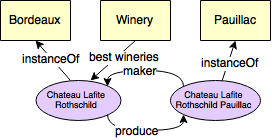
\includegraphics[width=.4\columnwidth]{graph/wine.png}
\caption{An example ontology for the domain of winery.}
\label{fig:wine}
\end{figure}
%\TODO{This is a bad example, not familiar domain with foreign names. Changed it to Person, Parents, Human etc to shown similar nodes and edge, matching the text later on}

% I want to quickly introduce DL and OWL.
The theory foundation of ontology is Description Logic (DL)~\cite{krotzsch2012description}, a family of formal knowledge representation languages for formal reasoning on the concepts of a domain. 
DL is expressive enough to build sophisticated knowledge bases while still supporting efficient inference.
It has a popular standardized dialect, Web Ontology
Language or OWL~\cite{mcguinness2004owl}. 
%Programming languages based on Description Logics (DL) are often used
%for representing an ontology~\cite{krotzsch2012description}. 
DL allows the use of {\em axioms} to describe a knowledge
base. For instance, an axiom \textsf{Person(Alex)} describes that
``Alex'' is an instance of class ``Person'',
and $\mathsf{Person}\sqsupseteq \mathsf{Human}$ describes the
subsumption relationship between concept \textsf{Person} and concept
\textsf{Human}. DL languages could use different
grammars. Conventionally, a simple yet uniform format to represent axioms is \textsf{(subject, property, object)} triple. Axioms in DL
languages can all be mapped to such a format. For instance, in
\textsf{Person(Alex)}, ``Alex'' is the subject, ``instance of'' is the
property, and ``Person'' is the object. Visually, it is an ``instance
of'' edge flowing from the ``Alex'' node to the ``Person'' node in an
ontology graph.

%For the generic form of knowledge representation offered by Ontology,
%automatic inferences on the knowledge of a domain becomes possible.
Through decades of development, a large body of tools 
(e.g., Stanford Protege~\cite{gennari2003evolution}, SWI-Prolog Semantic Web Library~\cite{wielemaker2011}, etc.)
%\TODO{add citations for DL reasoners such as SWI-Prolog, Pellet,
%Racer, FaCT++, HermiT, etc}
have been developed for creating ontologies and automatic reasoning upon an ontology-based
knowledge base, which enables automatic questions-and-answers,
consistency check of the knowledge base, derivation of new knowledge,
and so on.

Like declarative program analysis, most of these tools leverage logic
programming languages (e.g., Prolog) for inferences. In logical
programming, a program is composed of a list of rules written in the
form of \emph{clauses}:
\[
\mathsf{H \mbox{:-}  B_1, \dots, B_n.}
\]
which reads as 
\[
\textsf{H is true if } \mathsf{B_1} \textsf{ is true and ... } \mathsf{B_n} \textsf{ is true.}
\]

H is called the \emph{head} of the rule and $\mathsf{B_1, \dots, B_n}$
is called the body. When the body is empty, the rule
becomes \emph{fact} such as $\mathsf{variable(a)}$. 

%\TODO{Queries and how they are resolved by the underneath inference
%  engine of a logic language implementation.}







\section{Overview}
\label{sec:overview}
By offering a generic way to represent the knowledge in a domain,
Ontology simplifies the accumulation and share of various kinds of
knowledge among people or software agents. At the same time, it allows
automatic analysis and utilization of knowledge through high-level
declarative logic programming, thanks to its description logic
foundation.  These properties make it potentially valuable for
facilitating program analysis which is essentially about reasoning
about the knowledge related to a program. 

%% This section first gives an overview of the idea of using
%% ontology for program analysis. It then lists the critical challenges
%% for materializing the idea into a practical framework.

%\subsection{Overview}

\begin{figure}[t]
\centering
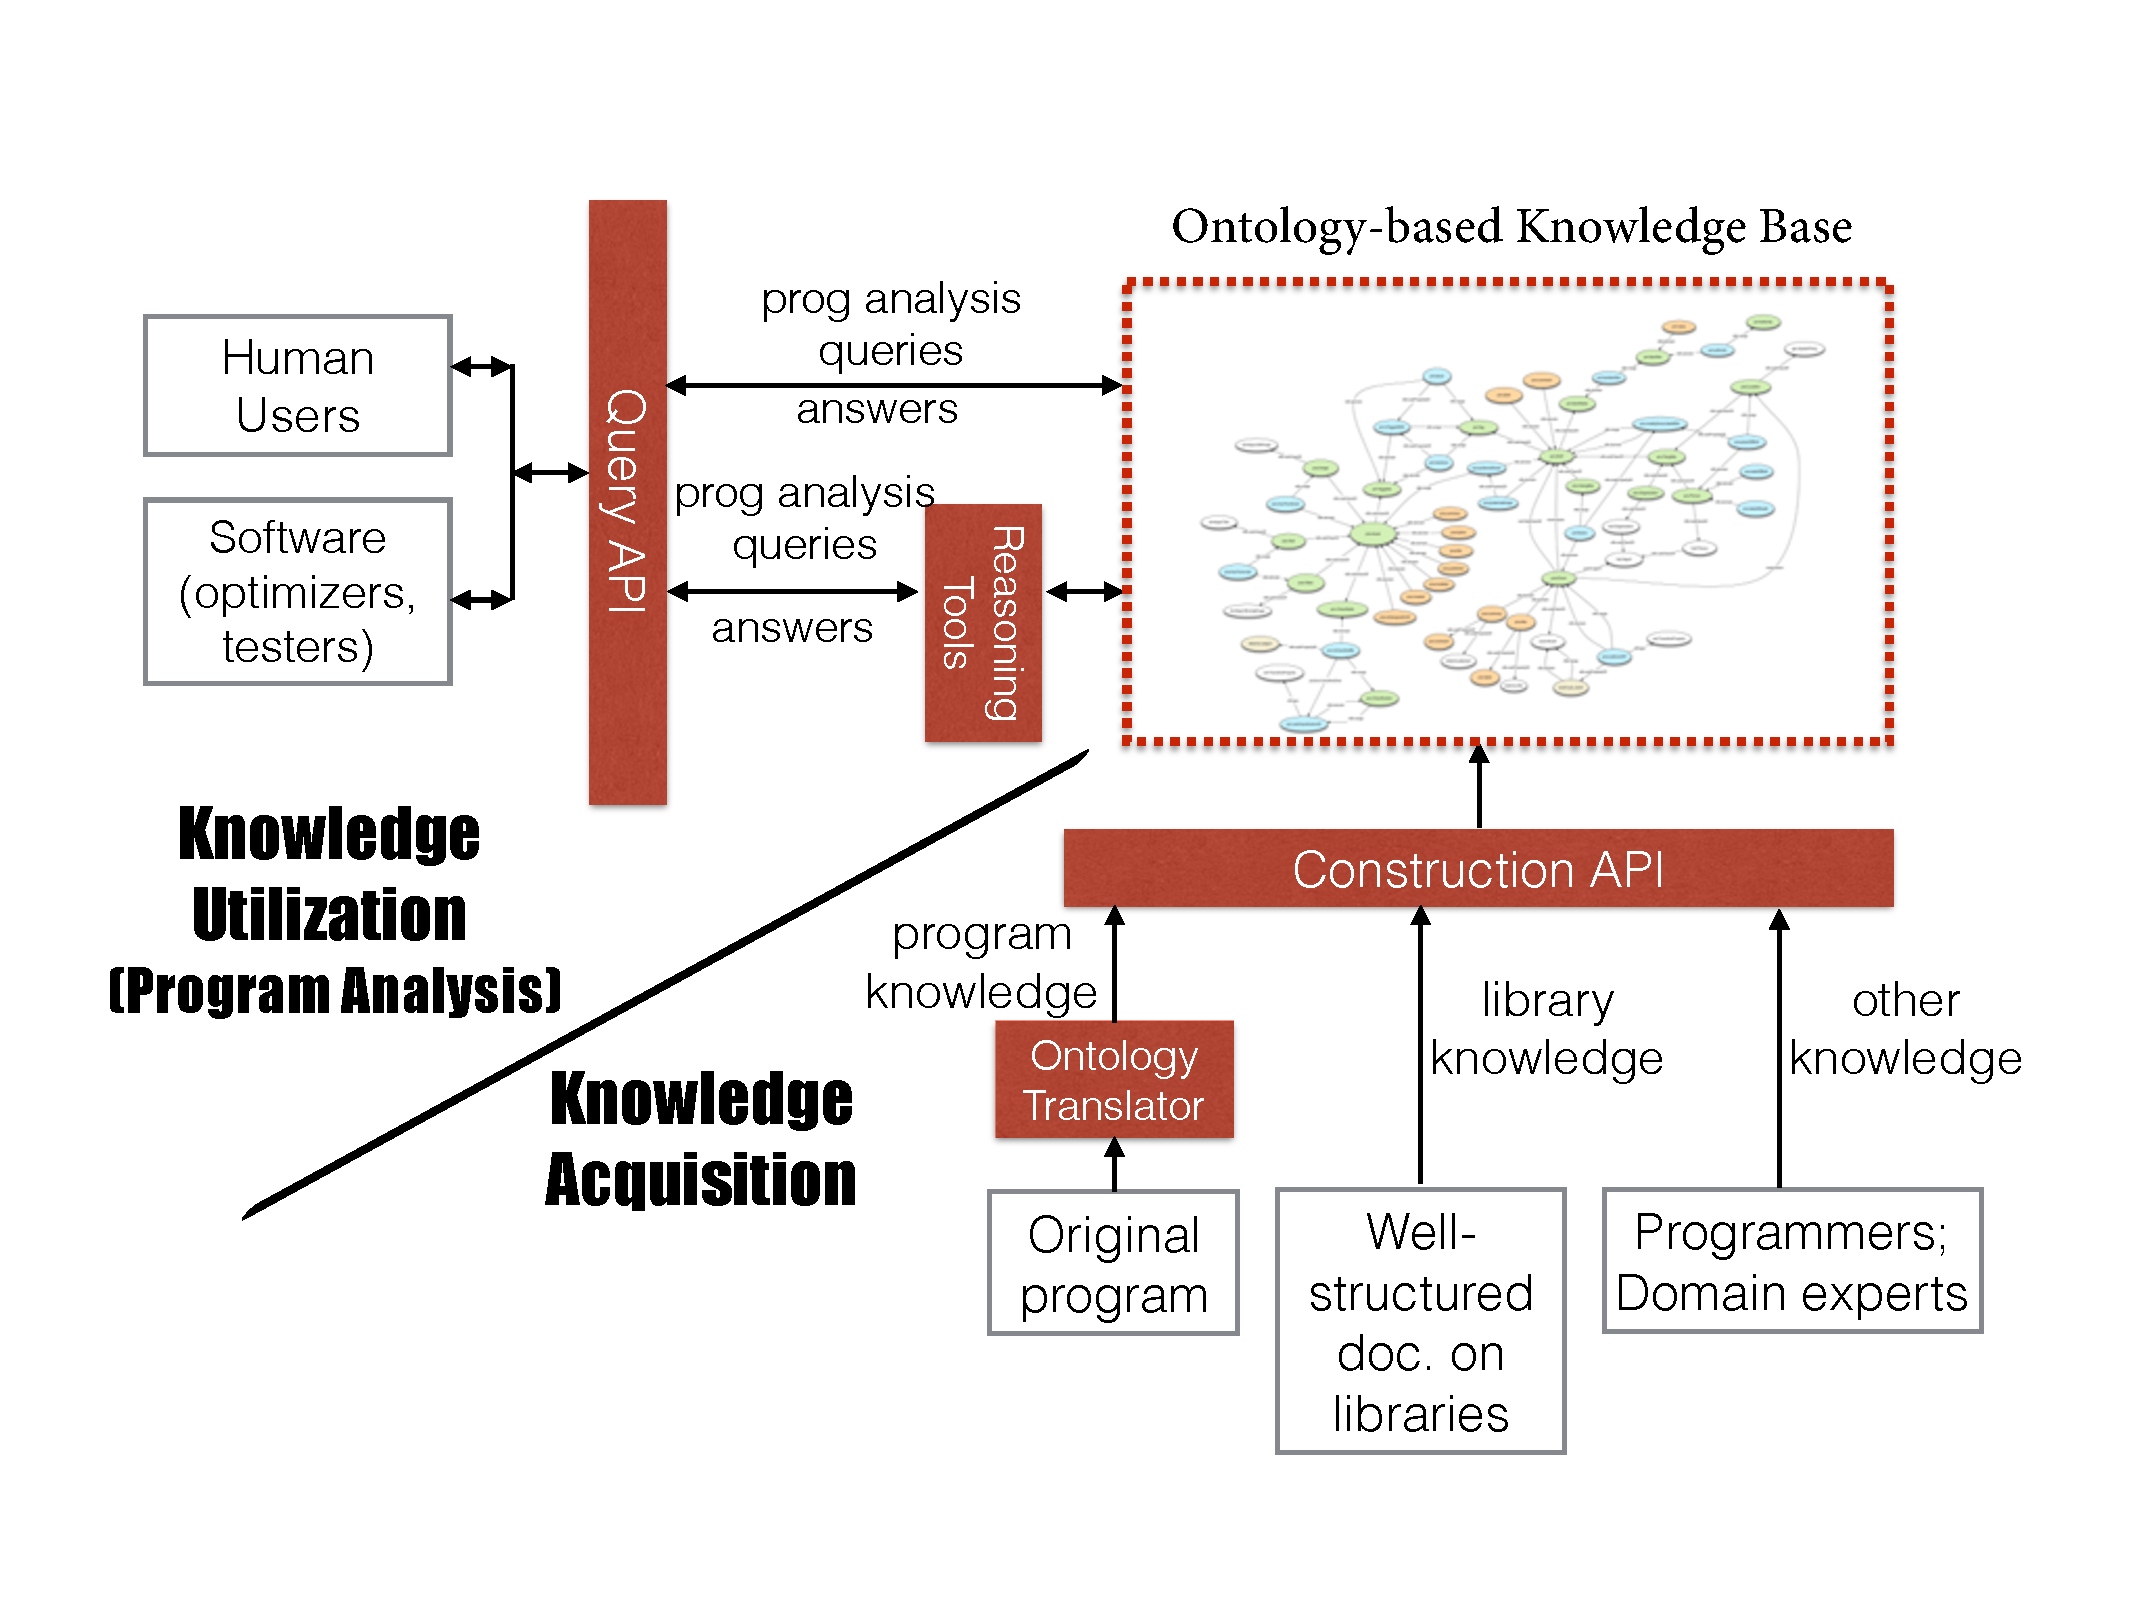
\includegraphics[width=.9\textwidth]{graph/overview.pdf}
\caption{Overview of using ontology for program
  analysis.}\label{fig:overview}
\end{figure}

Figure~\ref{fig:overview} illustrates the basic idea of ontology-based
program analysis. It centers around a knowledge base built upon
ontology.  The knowledge base may consist of the basic knowledge about
the code of the target program, as well as other knowledge (e.g.,
architecture attributes) relevant to the program analysis. An {\em
  ontology converter}, equipped with a parser, derives the basic
program knowledge from the code of the program, expresses the
knowledge in a standard format, and puts it into the knowledge
base. This basic knowledge may include the structures and components
(control blocks, data structures, etc.) of the program. In addition,
the knowledge base may include some knowledge that could be imported
about some libraries, or directly inputted by a domain expert on some
properties they know about the program or the architecture the program
is to run on (for the purpose of optimizations).

Built on top of description logic, ontology-based program analysis
keeps the conveniences of declarative program analysis. Rather than
writing thousands of lines of code inside a complex compiler, users
can simply write some logic queries about the kind of properties
(e.g., which loops are canonical loops) of the program that they want
to know. These queries should follow some ontology query APIs. The
APIs will then return the answers that are automatically obtained from
the ontology-based knowledge base. Processing of complex queries can
leverage many existing ontology reasoning
tools~\cite{wielemaker2011,tsarkov2006fact++}.  Users
of the ontology-based knowledge base can be humans as well as software
agents (e.g., tools for program optimizations or testing.)

\vspace*{.1in}
\noindent{\bf Example} We use canonical loop analysis to illustrate
how the idea of ontology-based program analysis works. A canonical
loop is a type of well-structured loop conforming to specifications as
shown in Figure~\ref{fig:canonical}.  Because of its regular
structure, it has been the focus of many studies on parallelization
and loop
optimizations~\cite{kandemir1999improving,LiaoSemantic-aware2010,DaMata2013}.

\begin{figure}[h]
\centering
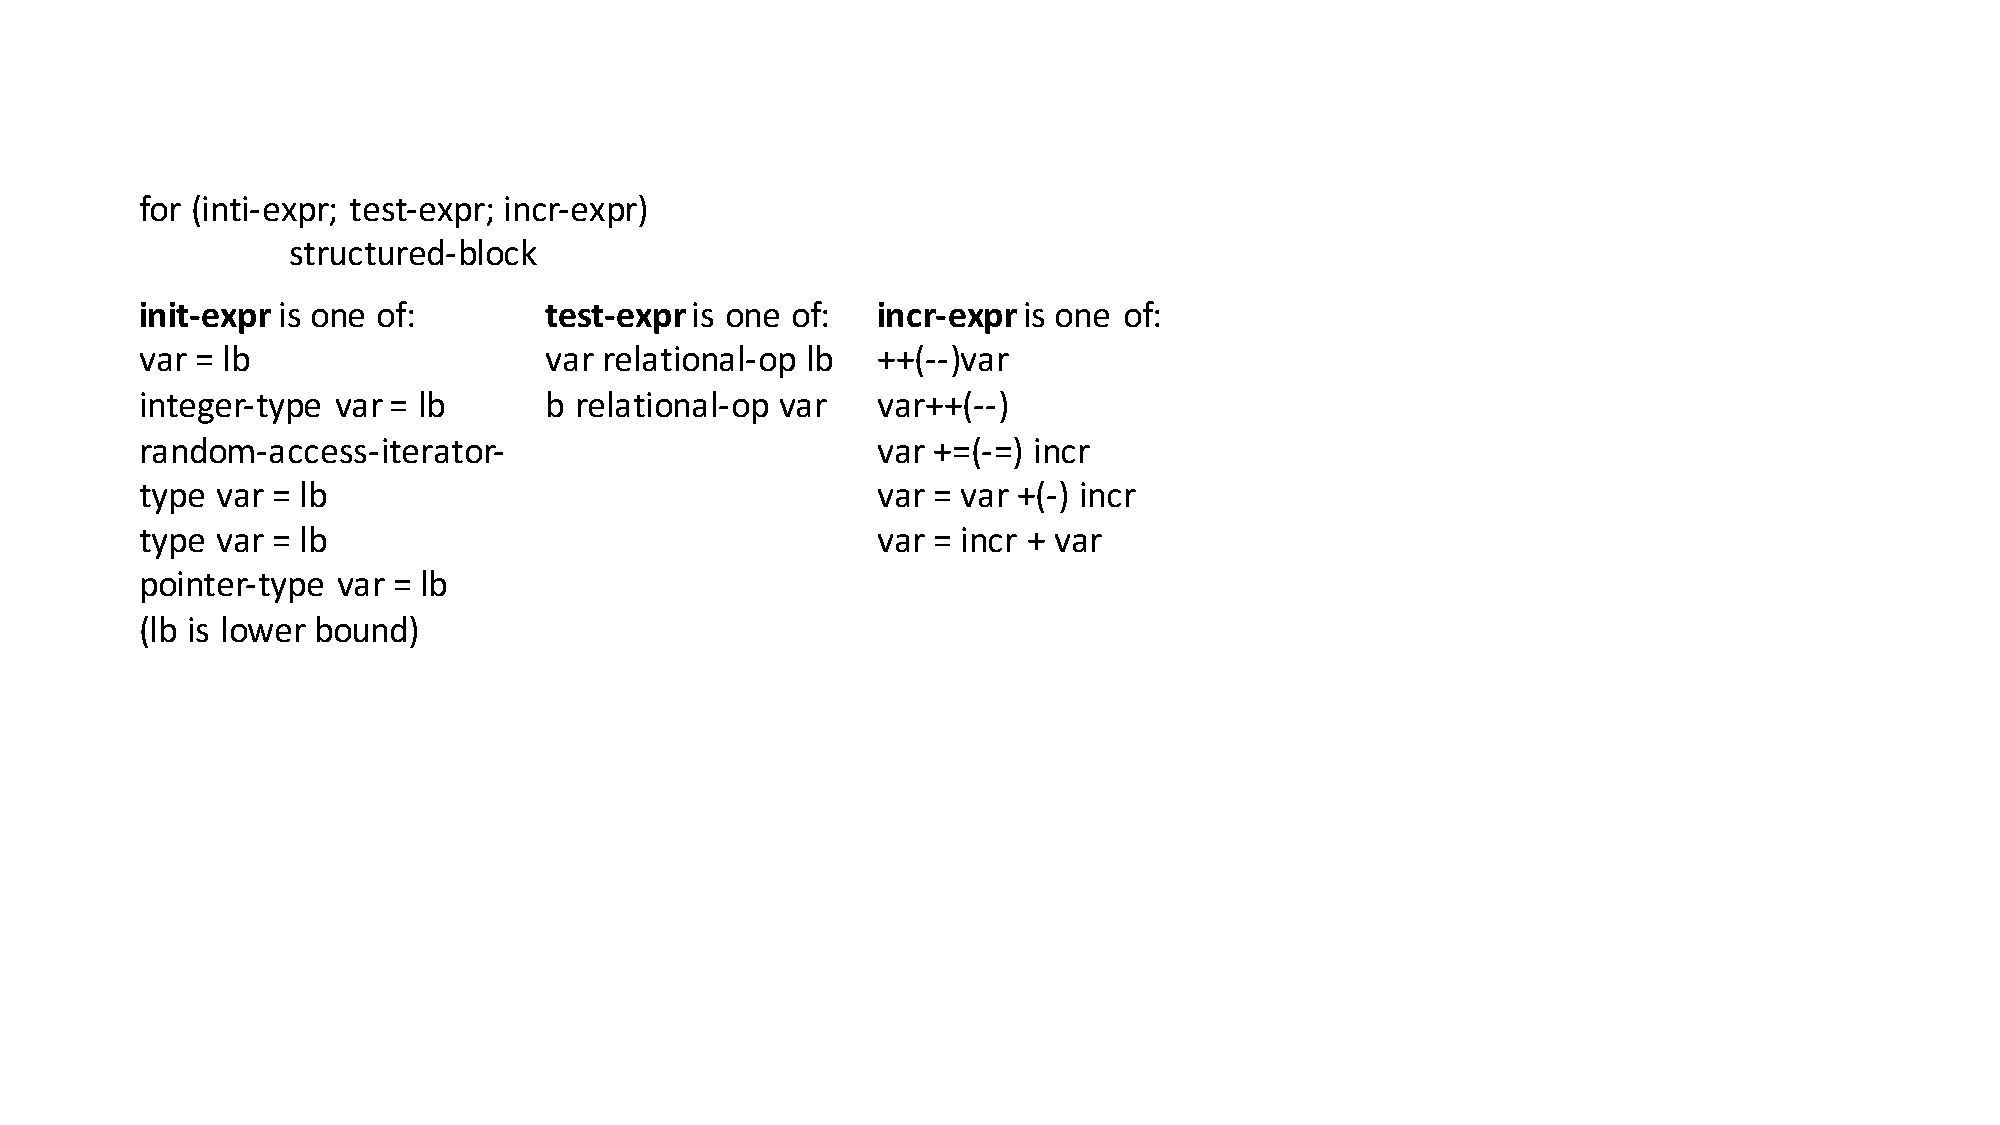
\includegraphics[width=.7\columnwidth]{graph/cl-def.pdf}
\caption{Specification of a canonical loop (derived from OpenMP
  manual~\cite{openmp13}.)
  %\TODO{remove boxes, put the three kinds of expr definitions into one single row below the ``for'' loop code.}
}
\label{fig:canonical}
\end{figure}

%An important program analysis (e.g., in ROSE~\cite{ROSE} and ??
%compilers)
The goal of {\em canonical loop analysis} is to recognize whether a
loop is in a canonical form.  Traditional implementations of the
analysis (e.g., the implementation in the ROSE compiler~\cite{ROSE})
contains hundreds of lines of code for examining the IR of a loop. The
code is tied to a particular internal data structure of the chosen
compiler, hard to port to another compiler or maintain.

In a
traditional program analysis development, the task requires an
insertion of a separate pass over some intermediate representation of
the whole program, which may need the development of thousands of
lines of code. For example, in the ROSE compiler~\cite{ROSE} (a
source-to-source compiler broadly used in High Performance Computing),
the pass works on an Abstract Syntax Tree (AST). To analyze the code
at that level, a programmer needs to implement many lines of code
written in procedural languages (C/C++).  The canonical loop analysis
in the ROSE compiler consists of 380 lines of source code for examining
the representations of the structure of each loop and check them
against the conditions in Figure~\ref{fig:canonical}.
%\TODO{add back the canonical figure using imperative codes}

In ontology-based program analysis, the process is simpler. The
programmer needs to invoke some provided ontology converter on the
code of the target program. An ontology-based knowledge base is then
produced to capture the program constructs, components, and their
relations.  The programmer then just needs to use a declarative logic
programming language to describe rules governing the forms that a
canonical loop should conform. Treating those rules as queries on the
ontology of the program, existing logic reasoners can then
automatically find all the canonical loops in the target program.
%\TODO{We should give sample ontology triplets and a few declarative analysis rules here. Otherwise readers cannot understand this.}
For example, a fragment of C code is shown in Listing~\ref{code:id}.
\begin{lstlisting}[numbersep=-8pt,firstnumber=0,
xleftmargin=.1\columnwidth,
xrightmargin=.1\columnwidth, float,
caption=Example C code fragment, label=code:id]
  // s.c
  int a = 0;
  int foo() {
   for (int i = 0; i < 10; i++) {
    a = a + i;
   }
  }
\end{lstlisting} 
The code's corresponding ontology representation is shown in Listing~\ref{code:onto_repr}.
Each line is a triple of a subject, a predicate and an object.
The numbers in the subjects are the line and column numbers for the begining and ending positions of a language construct in the source code. 
\begin{lstlisting}[xleftmargin=.1\columnwidth,
xrightmargin=.1\columnwidth, float,
caption=Sample ontology for C snippet, label=code:onto_repr]
('3:1,5:1', rdf:type, 'ForStatement')
('3:6,3:14', rdf:type, 'VariableDecl')
('3:6,3:10', rdf:type, Variable')
('3:1,5:1', 'hasForInit', '3:6,3:14')
('3:1,5:1', 'hasForTest', '3:17,3:22')
('3:1,5:1', hasForIncr', '3:25,3:27')
('3:1,5:1', hasBody', '3:30,5:1')
\end{lstlisting}
%\begin{lstlisting}[xleftmargin=.05\columnwidth, 
%xrightmargin=.05\columnwidth, float=h,
%caption=Sample ontology triples, label=ont:c_frag]
%...
%:334_3_342_3 rdf:type c:ForStatement .
%:334_3_342_3 c:hasParent :333_1_348_1 .
%:334_3_342_3 c:hasForInit :334_8_334_16 .
%:334_3_342_3 c:hasForTest :334_18_334_30 .
%:334_3_342_3 c:hasForIncr :334_33_334_38 .
%:334_3_342_3 c:hasBody :334_41_342_3 .
%... % omitted
%\end{lstlisting}
The different program constructs can be easily extracted by Prolog queries like those in Listing~\ref{code:sample_rule}.
\begin{lstlisting}[xleftmargin=.1\columnwidth,
xrightmargin=.1\columnwidth, float,
caption= Sample analysis rules, label=code:sample_rule]
isForStatement(Loop) :-
 rdf(Loop, rdf:type, c:ForStatement).
hasForInit(Loop, InitExpr) :-
 rdf(Loop, c:hasForInit, InitExpr).
\end{lstlisting}


Allowing the use of logic programming, ontology-based program analysis
inherits the productivity benefits of declarative program
analysis. More importantly, it overcomes the three aforementioned
shortcomings of existing declarative program analysis by leveraging
Ontology for standardizing the concept definitions in a domain and the
flexible representation of various sources of knowledge. 

%As
%shown in Figure~\ref{fig:loopProlog} (which will be further explained
%in Section~\ref{sec:exp}), the description can be nearly as simple as the
%English description in Figure~\ref{fig:canonical}. After that, the
%programmer just needs to put in a simple query in the Ontology Query
%API, asking the ontology reasoner to find all loops meeting the
%canonical loop conditions. The reasoner can soon return all the
%answers with the options of various visualizations of the results.

%% Writing declarative program analyses over an ontology is more
%% productive than writing imperative program analyses over a compiler
%% IR.  The main reason is that declarative programming interface works
%% on high level concepts.  It is quicker to develop and easier to make
%% it right. In addition, it is easy to modify and extend; some updates
%% to the high-level descriptions would be mostly sufficient.  It is also
%% portable since the concepts and relations being operated upon are
%% generic terms in the domain, totally independent from any particular
%% compiler's internal data structures.

%% Although the idea of the new paradigm is relatively straightforward,
%% materializing it is much beyond a simple application of the Ontology
%% techniques. There are some open questions special to program analysis that
%% must be answered. We present them and our next section.



%\section{Challenges, Solutions, and PATO}
\section{Challenges and Solutions}
\label{sec:solution}
The challenges for integrating Ontology into program analysis exist in
each of the four main steps: the design of an ontology for the domain,
the generation of the knowledge, the utilization of the knowledge
base, and the design of the entire framework.  In this section, we
discuss each of the challenges and present some principles we use to
address them. At the end, we describe PATO, 
the prototype framework we have developed to do ontology-based program
analysis.  % that we have developed in this work.

\subsection{Ontology Design}

\vspace*{.1in}\noindent {\bf Challenges} To create an ontology for any
domain, the first primary task is to define the vocabulary to be used
in the domain. That includes the definition of the concepts,
properties, and restrictions in the domain.
These definitions establish the conceptual
terms and their relations of the ontology-based knowledge base for the domain.
Even though there are some de facto procedures on
designing an ontology~\cite{noy2001ontology}, program analysis has
some special challenges. %Unlike some other domains that has only
%several predefined kinds of tasks (e.g., navigation of a robot),
Program analysis has a large variety of tasks (e.g., loop analysis,
data access pattern analysis, alias analysis, dependence analysis,
liveness analysis, busy expression analysis, etc.) involving a huge
set of diverse concepts and relations.  Even a larger variety exists
in the input programs.  So the first question to use Ontology for
program analysis is how to design an intuitive, efficient and flexible
ontology that can facilitate the various program analyses and input
programs.

\vspace*{.1in}\noindent {\bf Solutions} 
Through our explorations, we have found the following three principles
helpful.

%\begin{itemize}
%\item
{\em Language standard-oriented design.}  When designing the
vocabulary of an ontology, it helps if one starts with reusing
language constructs and their categorizations defined in the standard
of the programming language of the target programs. Despite the
variety of the input programs, they are all artifacts following the
particular programming language. With the constructs and their
categorizations of the programming language covered, we can easily
express programs using the language in the ontology-based knowledge
base. This approach helps achieve a good coverage of the input
programs with familiar vocabulary for users.  For example, to model C
programs in an ontology, we followed the standard of C99 and enumerate
all program constructs and concepts in a top-down
fashion. Figure~\ref{fig:c_onto} shows a fraction of the top-level
ontology for C programs.  The main concepts in the domain include
variables, expressions, statements, and so on. The ``construct'' on the
edges indicate these vocabularies are the basic constructs in the C program domain.

%Examples of concepts include
%types, linkage of identifiers, name spaces of identifier, and so
%forth. 
\begin{figure}[h]
	\centering
	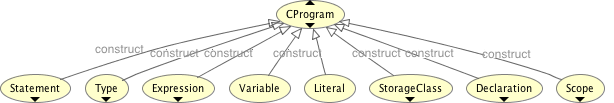
\includegraphics[width=\columnwidth]{graph/c_onto}	
	\caption{Top-level ontology for C program analysis.
		%\TODO{}
		}
	\label{fig:c_onto}
\end{figure}

%\item
{\em Being generic in property designs.}  Besides classes of concepts,
an ontology also contains a vocabulary for properties (or called
relations).  For example, an \textsf{Expression} instance may have
some \textsf{Type}, an \textsf{Identifier} may refer to some
\textsf{Definition}. Because there may be many properties to express,
in our practice, we follow a principle trying to define properties in
a generic way, and encode semantic meanings into concepts whenever
possible.  That allows the possible use of a small set of properties
and their combinations to express a large number of possible
properties in a program. For example, when describing \emph{an
  identifier has static storage class}, one approach is to define a
property \textsf{hasStaticStorage} and use it like \textsf{(someVar
  hasStaticStorage true)}.  Alternatively, we may define the concept
\textsf{Storage} as a class and use a simpler property
\textsf{hasStorage} as \textsf{(someVar hasStorage static)}, where
\textsf{static} is a member of \textsf{Storage}.  There are several
benefits for this second choice. First, using generic properties makes
the set of property vocabularies small and thus easy to manage.  For
example, \textsf{hasStorage} is used to describe all storage classes
instead of creating specific properties for each storage class.
Second, stripping semantics from property make writing logic rules
more flexible.  For example, the knowledge of \textsf{(someVar
  hasStorage static)} can be queried by the keyword
\textsf{hasStorage}.  Otherwise, users may need to use many specific
keywords as \textsf{hasStaticStorage}, \textsf{hasExternStorage}, and
so on.

%\item
{\em Continuous enrichment.}  In our exploration, we find that
continuous enrichment of the ontology vocabulary can be helpful. For
instance, in a canonical loop analysis, a user gives the description
of the concept of a canonical loop.  If that concept turns out to be
needed frequently (by many users), the concept could then be
integrated into the ontology framework to save the need for repeated
descriptions. Given that the program analysis ontology is intended to
be used by a community, a complexity is that different users may use
different names for a single user-defined relation (e.g., canonical
loop), making the detection of the repeated use of a user-level
concept difficult. Ontology-based logic reasoners come in handy. As the
descriptions of user-defined relations all use the vocabulary in the
same ontology, the reasoners can easily do a logic reasoning on the
descriptions to decide whether two user-defined relations are
equivalent. After recognizing the frequently needed user-level
concepts, such concepts can be added into the standard ontology for
future reuse.  
%Another benefit of such a feature is to support program
%analysis that requires some additional concepts that are not covered
%by existing vocabulary.
%\end{itemize}

Based on the three principles, we came up with an Ontology for C
program analysis, containing 178 concepts and 68 properties. It is not intended to be complete, but is sufficient for
examining the support of a single ontology to multiple different
program analyses as we will show later in this paper. 

\subsection{Knowledge Generation} % Knowledge Base Construction 

\vspace*{.1in}\noindent {\bf Challenges} 
Building up a knowledge base is essential for any application of
Ontology. For program analysis, the knowledge base shall include the
important knowledge related with the to-be-analyzed program. There are
three main questions to answer.  {\em (1) Ontology converter.} How to
construct an ontology converter that can automatically convert a given
program into the Ontology representation needed by many common program
analyses.  {\em (2) Naming.}  A program may contain functions,
statements, expressions, variables, and so on.  Any of them may appear
many times in difference locations. A challenge is what naming scheme
the ontology should use to reference each reference to avoid
ambiguity. {\em (3) Mapping.} One of the objectives of ontology-based
program analysis is to facilitate the cooperations among different
compilers and other program analysis tools. A difficulty is that they
may have different internal representations of a program.  To make
them able to interact based on the program ontology, the instances of
program constructs in the knowledge base should be possible to map to
some common ground meaningful to the different tools. One intuitive
choice of such common ground would be the source code of the
program. That will also make it easy for human to collaborate with
program analysis tools.  A complexity in using source code for
references is how to make the naming robust to code changes.  {\em (4)
  Space.} The knowledge about a program can be tremendous. Besides the
basic knowledge directly driven from the program, there could be many
other higher-level knowledge such as canonical loops, data dependences
among statements, and so on. This higher-level knowledge is derivable
from the lower-level knowledge. The derivation through reasoning may
take non-trivial time. But if all this knowledge is saved in the
knowledge base, the space cost could be large. How to strike a good
balance is important for practical usage of this new program analysis
paradigm.

\vspace*{.1in}\noindent {\bf Solutions} 
We come up with the following solutions to these
challenges. 

%\begin{itemize}
%\item
{\em Ontology converter.} Our experience shows that an ontology
converter can be easily created by building a translator on top of a
source-to-source compiler such as ROSE~\cite{ROSE}.  A
source-to-source compiler usually produces an abstract syntax tree
(AST) representation which is close to the input code. The translator
traverses the AST of the program to get structural and semantic
information, which is then stored into the knowledge base as
ontology. The program constructs are represented as individuals
(i.e. instances) of some of the classes defined in the language
ontology. Relations between them are represented by properties.
%The translator can be reused (with certain extensions) across programming languages as long as they use the same or similar form of AST. 

%\item
{\em Naming and Mapping.} 
In our naming scheme, we borrow the internationalized resource
identifiers (IRIs)~\cite{hitzler2009owl} that OWL uses. It helps avoid name conflicts. 
For the ontology of C program language, names of concepts are built directly from the corresponding terms used in the C language standard.
\footnote{We follow the naming convention of \textsf{UpperCamelCase}
  for classes and \textsf{lowerCamelCase} for properties.}  For
example, the concept \textsf{type} is referenced as \textsf{c:Type}.
An example IRI for the concept of types in a C program domain can look
like ``http://example.com/owl/CProgram:Type''.  Some alias can be
defined as short names for the prefix strings of a domain.
%We have an alias \textsf{c} for our C
%language domain. 

More care needs to be taken for designing the naming scheme for
representing the instances of a program construct.  Named constructs
such as types, variables, functions can use the C++ qualified name
concept to uniquely identify them.  For an unnamed construct (e.g. an
assignment statement) or a reference to named construct (e.g. variable
reference), a common intuitive approach is to use its location in the
source code of the program, such as $ \mathsf{file\ url,
  start\ location,end\ location} $ where the location is a pair of
(\textsf{line number}, \textsf{column number}). For instance,
``http://my.com/file1.c, 3:1, 5:1'' could refer to a loop that spans
from the beginning of the third line to the beginning of the fifth
line of file1.c. The problem with this scheme is that some minor
changes to the original program may invalidate all the names of the
constructs after the modification point.

We find {\em scoped IRI} useful to restrict the impact of a code
change to the names.  In {\em scoped IRI}, a name is composed of some
qualified names and some relative locations in the source code. For
constructs like functions, structures, global variables, we add their
scopes before their names. Other constructs within these constructs
are named by their locations, while the line numbers are relative to
the start line number of their surrounding constructs rather than the
beginning of the source-code file. Using this method, a global
variable declared in the first line of a file ``s.c'' (from column 5
to 6) can be named as \textsf{s.c::1:5,1:6}, while a variable declared
on the first line inside a function foo in file ``s.c'' (from column 6
to 10) can be named as \textsf{s.c::foo()::1:6,1:10}.  Thus, if there
is some change of the code, only the names in the same scope as the
changing point need to be updated.

%\item
{\em Space.} 
%Besides the basic knowledge on the program code,
%  there can be a lot of other relevant knowledge coming up in program
%  analysis. Due to the large variety of programs and relevant
%  analyses, saving all of them into the knowledge base could cause
%  space issues. 
To address the space challenge of putting everything into a knowledge
base, we split the knowledge base into a core knowledge base and
multiple loadable supplemental knowledge bases.  The core knowledge
base is always loaded and others are loaded as needed.  We also design
a cache-like management mechanism to alleviate the problem. It
maintains a buffer to store derived supplemental knowledge. When the
upper limit of the buffer gets reached, it starts to evict some of the
stored knowledge.
  %Here, the eviction
  %means removing the knowledge but keeping the commands for deriving
  %the knowledge such that when needed, the knowledge can be derived
  %quickly. 
  For the eviction policy, there can be multiple choices:
  least-recently-used (LRU), least-frequently-used (LFU), and their
  variants that are weighted with the size of the knowledge. 
  %We are
  %not aware of such solutions used in previous ontology-based systems
  %(in other domains).
%\end{itemize}

\subsection{Knowledge Utilization}

\vspace*{.1in}\noindent {\bf Challenges} Some challenges also exist in
the utilization of the knowledge base for program analysis.  {\em (1)
  Efficiency.}  In many cases (e.g., analyzing a large program), the
runtime efficiency of conducting a program analysis could be
important. A question to answer is whether the improved productivity
of the new paradigm hurts the runtime efficiency and if so, how to
improve the efficiency. {\em (2) Generality.}  Using descriptive
programming languages could be awkward for some usage cases,
especially when they involve some mathematical computations. Such
cases however do exist in some program analysis and optimizations, for
instance, when they relate with some performance models (an example is
the data placement optimizations Section~\ref{sec:exp} will
describe). Effectively overcoming such limitations is important for
the general applicability of ontology-based program analysis.

\vspace*{.1in}\noindent {\bf Solutions} We address these issues by
both creating some shortcuts and leveraging features of existing
ontology tools.

{\em Efficiency.}  Recent years have seen some significant improvement
of the performance of logic reasoners~\cite{tsarkov2006fact++, bassiliades2006defeasible}. 
%\TODO{cite some papers; see the related work section of some of Kemaphor's paper} 
  Many
optimizations have been developed.  For instance, in SWI-Prolog, the
ontology is stored as relation triples of \textsf{(subject property
  object)} with C extensions and some indices are built for each
element in the triples.  So a search of a particular element can be
done in constant time.  Additional optimizations can be applied to
queries.  For instance, Prolog provides the \emph{cut} operator (i.e.,
the ! symbol) to avoid unwanted backtracking in search. We find that
following some existing guidelines when writing
queries~\cite{Bratko2000} can be quite helpful for quickly
narrowing down the reasoner's search space.

In scenarios where the relevant knowledge base is simple and consists
of straightforward facts in triples (e.g., some memory
configurations), one may construct a customized lightweight parser in
high performance languages, which can further help achieve good
performance than going through a heavy-weight logic reasoner.

%\item
{\em Generality.} Ontology-based logic reasoning meets the needs of
many typical program analyses, but is not immediately natural for
expressing analyses that involve a lot of mathematical computations
(e.g., a regression-based performance modeling).  We find that a
mechanism called \emph{computable}~\cite{tenorth2009knowrob} in
Robotics can help resolve the issue. Computable is some special
ontology entity that can attach procedures to some classes or
properties.  When the deduction rule queries the individuals of one of
the classes or the properties, the associated procedures is invoked to
compute individuals for the target class or property. The procedure
can be written in a wide range of programming languages (e.g., C, C++,
Python).
%\end{itemize}

Besides allowing the direct input of queries by users written in logic
programming languages, ontology-based program analysis also allows
queries coming from a third-party software (which could be written in
even imperative languages like C, C++ or Java.) For such cases, the
ontology can be processed with libraries for those languages (e.g.,
the OWL API~\cite{horridge2011owl} or Prolog interface to foreign
languages\cite{bagnara2002foreign}). That offers the conveniences for
existing software tools (e.g., a compiler) to easily leverage a
program analysis ontology.


\subsection{Framework Design and PATO} 

The final challenge is how to organize the various components together
into a unified framework for program analysis. It includes choosing
the DL language and the reasoner that suit the needs of program
analysis, designing and implementing the APIs for both knowledge base
construction and queries, and integrating all the components together
into a complete cohesive framework that offers effective support to
various program analyses. 

\begin{figure}[ht]
\centering
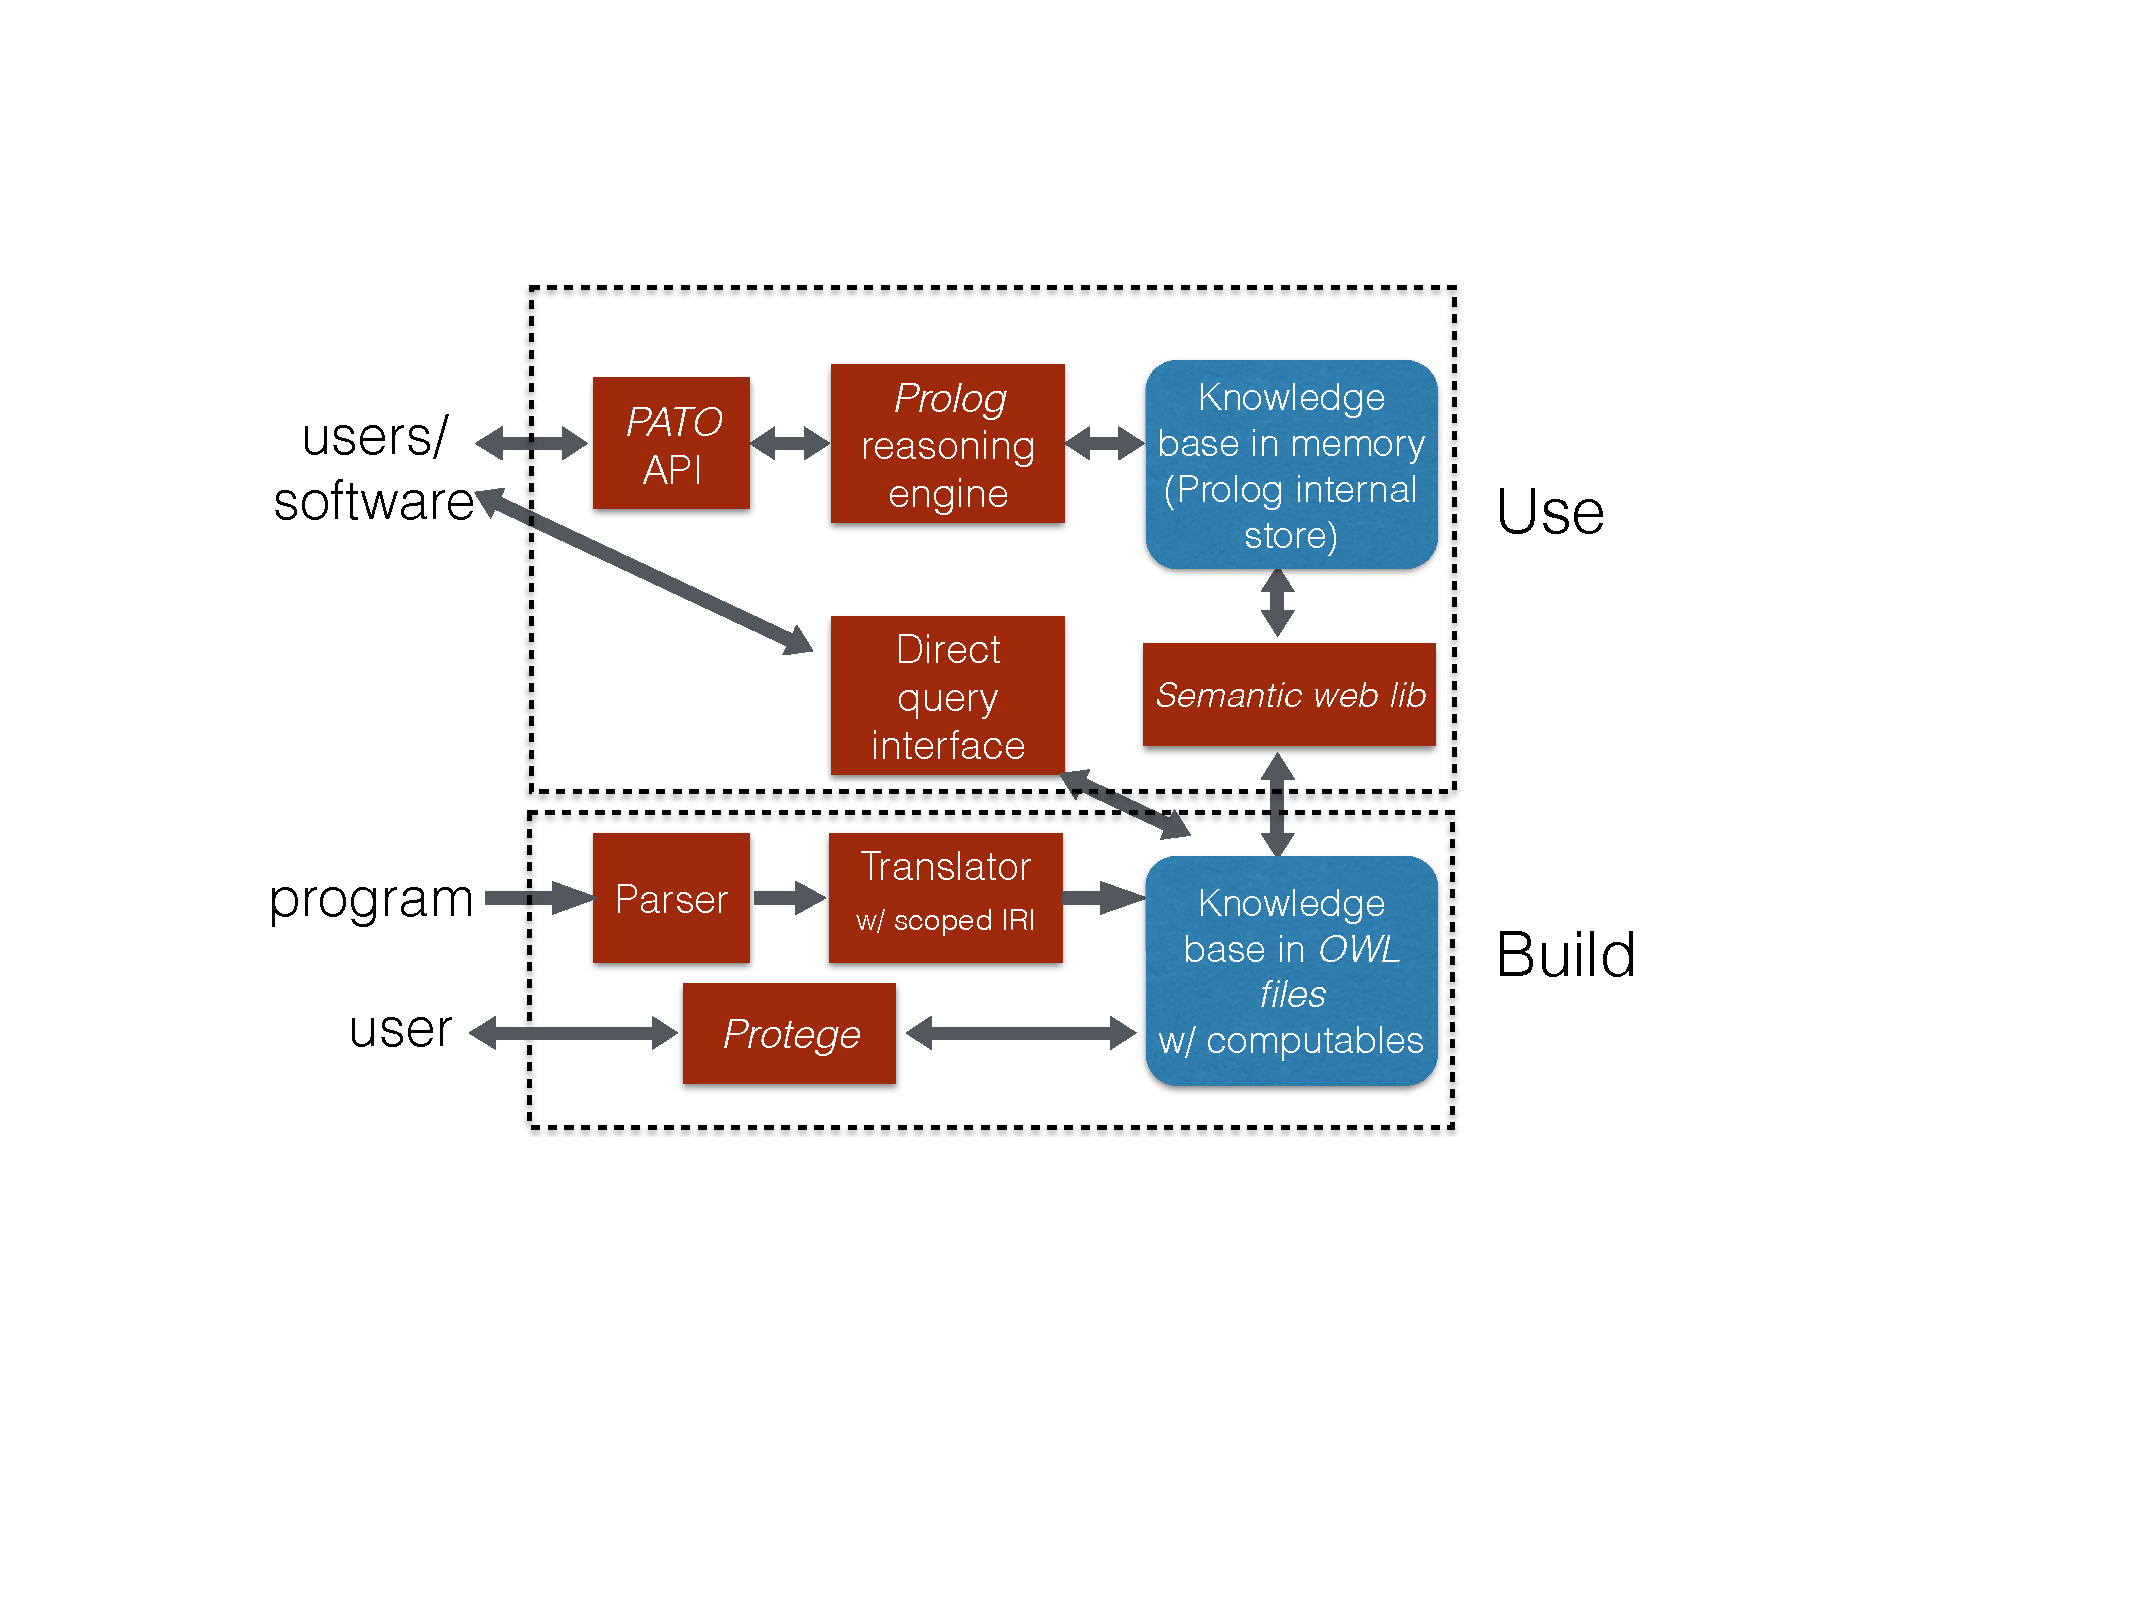
\includegraphics[width=.7\columnwidth]{graph/patoDiagram.pdf}
\caption{Structure of PATO.}
\label{fig:pato}
\end{figure}

To answer these questions, we have developed a prototype framework
named PATO for ontology-based program analysis. It integrates all the
aforementioned solutions to the various challenges, and leverages the
power of existing ontology tools.

Figure~\ref{fig:pato} outlines the main components of PATO. The
knowledge base in PATO can be in two forms, represented by the two
round-corner boxes on the right part of the figure. On the disk, the knowledge is stored as OWL files.
Each entry in the files is in an
OWL triple \textsf{(subject, property, object)}. For instance,
\textsf{(var1, hasValue, 0)} means a variable has a constant value of 0. The
reason for selecting this form is that OWL triple are
 one of the standard
(and space-efficient) formats for ontology representations and is
accepted by many Ontology tools. Another part of the knowledge base is
the {\em computables}, which are attached to the concepts and
properties in the triple collection. The cache-like buffering mechanism
is used to help with the space efficiency of the knowledge base.

Two of the primary ways to add knowledge into the knowledge base are
shown at the bottom of Figure~\ref{fig:pato}. In the first way, there
is a parser (based on ROSE~\cite{ROSE}) to convert an input program code into an AST preserving source level information. 
%The parser
%is currently only for C programs, but parsers for other languages can
%be easily plugged into the framework. 
We have also developed a translator
which translates the basic program knowledge on the AST into OWL 
triples and stores them into the knowledge base. During the
translation, the translator uses the scoped IRI (described in the
previous section) as the naming scheme. In the second way, we adopt
Stanford Protege~\cite{gennari2003evolution}, an interactive tool for ontology creation and manipulation.
Through its GUI, a user can intuitively add
entries into the knowledge base. The plugins of Protege
also provide many other features to the users, such as visualization, validation, and querying. 

There are two ways to use the knowledge base. In the first approach
(on top of Figure~\ref{fig:pato}), we incorporate the SWI-Prolog
reasoning engine. As the engine for a mature logic programming
language, it has been continuously enhanced in the last few decades in
efficiency, generality, and reliability. At the beginning of a usage,
the OWL files are loaded into memory, during which process, they are
converted into an internal knowledge base through the existing Semantic
Web Library. The in-memory organization of the
knowledge base features some efficient indexing schemes as mentioned
in the previous section and hence offers good efficiency.  When seeing
a query from a user or software agent, the Prolog engine would start
working on the internal knowledge base to provide the answers.  Prolog
provides a general interface for input logic rules and queries. We
have further developed a higher-level set of API tailored to represent
some common terms used in program analysis tasks (e.g., loops,
functions, etc.), through them, the users may write even more concise
descriptions.

The second approach to use the knowledge base is shown as the shortcut
(the diagonal path) in Figure~\ref{fig:pato}. Through a direct query
interface we have developed in C++, the user or software agent may
directly work on the OWL file collection (and computables) without
going through Prolog which may not be available to a user or too
costly to use in some special scenarios. For tasks which only need
some simple fact search (without the need for much reasoning), this
approach is more efficient than the Prolog-based approach because it
avoids the overhead in Prolog interpretation and other associated
cost.  Both the Prolog and the shortcut approach can insert new
knowledge (e.g., derived in a previous program analysis) into the
knowledge base.

%% The semantic web library provides a set of built-in rules for queries
%% like
%% \begin{itemize}
%% 	\item \emph{rdf(S, P, O)} returns the matching triple store.
%% 	\item \emph{rdf\_has(S, P, O)} considers the \emph{rdfs:subPropertyOf} relation of Predicate.
%% 	\item \emph{rdf\_reachable(S, P, O)} additionally follows the transitivity of predicate.
%% \end{itemize}
%% and our custom query rules are built upon these basic rules. For
%% example, the query rules in Listing~\ref{code:init}.

%% OpenK framework offers a rich set of the query rules as part of the
%% API for program analysis. Due to the modular design, new APIs are
%% added incrementally and easily. Although the query APIs are in Prolog
%% program, they can be used in C, C++, Java via the SWI-Prolog Foreign
%% Language Interface.

%user input via interface (file? interactive interface)

%% To represent the program construct individuals, we need to design a
%% portable and human readable ID first. A common approach is to use the
%% code location for source-level names. To accurately separate each
%% construct, we can name the ID in the form of
%% $$ \mathsf{start\ location,end\ location} $$ where the location is a
%% pair of (\textsf{line number}, \textsf{column number}).

%% % illustrate the ontology of program

%% The ontology of input code is built with the vocabularies defined in
%% the C program ontology. For example, when declaring membership of
%% constructs, the classes must be defined in the C ontology. Properties
%% of these constructs must be from the C ontology too. Here is a
%% fragment of C code

%% \begin{lstlisting}[numbersep=-8pt,firstnumber=0,caption=Example of ontology naming, label=code:id]
%% // s.c
%% int a = 0;
%% int foo() {
%%  for (int i = 0; i < 10; i++) {
%%   a = a + i;
%%  }
%% }
%% \end{lstlisting} 
%% and the snippet of ontology representation for the loop is
%% \begin{lstlisting}[caption=Ontology representation for the C snippet, label=code:onto_repr]
%% ('3:1,5:1', rdf:type, 'ForStatement')
%% ('3:6,3:14', rdf:type, 'VariableDecl')
%% ('3:6,3:10', rdf:type, Variable')
%% ('3:1,5:1', 'hasForInit', '3:6,3:14')
%% ('3:1,5:1', 'hasForTest', '3:17,3:22')
%% ('3:1,5:1', hasForIncr', '3:25,3:27')
%% ('3:1,5:1', hasBody', '3:30,5:1')
%% \end{lstlisting}

%% In the example, the \emph{for loop} is assigned with the id
%% \textsf{3:1,5:1}. It is described by the property as being a member of
%% the class \textsf{ForStatement}. It is also described as consisting
%% four components, namely, the declaration \textsf{int i = 0}, \textsf{i
%%   < 10}, \textsf{i++} and the for body. All of them are named with
%% their code location. This naming convention guarantees uniqueness and
%% also make it easy for human to locate the constructs.

%% However, if the original program is modified, all names of constructs
%% after the modification point must be updated. It is thus not portable,
%% especially when the ontology is used for code transformation. This
%% location-based naming method can be improved. Our solution is to use
%% qualified names and relative location-base names: for constructs like
%% functions, structures, global variables, we add their scopes before
%% their names. It is similar to the C++ qualified name. Other constructs
%% within these constructs are named by their location but the line
%% numbers are relative to the start line number of their surrounding
%% constructs. Using this method, the global variable \textsf{int a} in
%% Listing~\ref{code:id} is named as \textsf{s.c::1:5,1:6} and the variable
%% \textsf{int i} can be named as \textsf{s.c::foo()::1:6,1:10} (the
%% original is \textsf{3:6,3:10}). Thus, if there's some change of the
%% code, only small part of the code is needed to update.





%% \section{Implementation details}
%% \label{sec:impl}
%% some parts in Section 5 of the previous version.



\section{Experiments}
\label{sec:exp}
Based on PATO, we conduct a series of experiments. To examine the
feasibility of using a single ontology to support multiple different
program analyses efficiently, we implement four types of program
analysis on PATO: canonical loop analysis, control flow graph
construction, data access pattern analysis, and GPU data placement
guidance. They differ in domains, relations, scopes, and intended
usage. Using GPU data placement optimization, we examine whether
ontology can indeed enable seamless linkage of various sources of
knowledge (programs, domain experts, and hardware) and whether
ontology-based program analysis can actually help guide program
optimizations. Using the liveness analysis on two compilers
(ROSE~\cite{ROSE} and LLVM Clang~\cite{Lattner2004}), we
examine the easiness of ontology for promoting cooperations among
different analysis tools. We next report our observations in each of
the experiments.

For the interest of space, our description concentrates on the 
canonical loop analysis and the GPU data placement guidance,
and briefly covers the other two program analyses.

%%%%%%%%%%%%%%%%%%%%%%%%%%%%%%%%%%%%%%%%%%%%%%%%%%%%%%%%%%%%%%%%%%%%%%%%%%%%%%%
\subsection{Canonical Loop Analysis}
%\TODO{description based on the Page5 rightside and P6 leftside of the
%  previous version (main\_ws.pdf); clarity needs to be improved; add the part on
%  iterators to show the easy tool-human synergy allowed by the new
%  paradigm}

%We use canonical loop analysis as the first example to evaluate the benefits of PATA. 
To help readers get a concrete understanding of using logic programming
for ontology-based program analysis, we first explain the Prolog code
for canonical loop analysis in a certain degree of detail. 

As mentioned earlier, canonical loop analysis (CLA) checks whether a
loop is in a predefined canonical form.  CLA is a fundamental analysis
to enable various loop
optimizations~\cite{kandemir1999improving,LiaoSemantic-aware2010,DaMata2013}.
%There are different specifications of what a canonical loop should
%look like.
In particular, we use the \emph{canonical loop form} defined in the OpenMP specification \cite{openmp13} as an example, shown in Figure~\ref{fig:canonical}.  
The specification of an OpenMP canonical loop can be written as declarative Prolog rules as shown in Listing~\ref{code:iscl}.
We use italic font to distinguish variable from normal symbols.

\begin{comment} % redundant figure, remove it
\begin{lstlisting}[xleftmargin=.1\columnwidth,xrightmargin=.1\columnwidth,
caption=Specification of an OpenMP canonical loop, label=code:cldef]
  for (init-expr; test-expr; incr-expr) structured-block
% init-expr is one of:
var = lb
integer-type var = lb
pointer-type var = lb
...
\end{lstlisting}
\end{comment}
%where every loop component has detailed specification (shown in Figure~\ref{fig:canonical}) .
%The above specification can be mapped to the logic rule of
%\begin{equation*}
%\begin{split}
%\text{is-a(canonical loop)} & := \text{has-a(inti-expr)} \wedge \text{has-a(test-expr)} \\ 
% & \wedge \text{has-a(incr-expr)} \wedge \text{has-a(block)}
%\end{split}
%\end{equation*}

\begin{lstlisting}[basicstyle=\ttfamily\footnotesize,
float=h, caption={Prolog specification of an OpenMP canonical loop
(italic upper-case for variables, lower-case for properties)},
escapechar=@, 
 label=code:iscl]
% top level rule to find canonical loop
canonicalLoop(@\emph{Loop}@) :- 
 isForStatement(@\emph{Loop}@), !, %'!' prevents backtracking
 hasForInit(@\emph{Loop}@, @\emph{InitExpr}@), %',' means logic AND
 canonicalInit(@\emph{InitExpr}@, @\emph{LoopVar}@),
 hasForTest(@\emph{Loop}@, @\emph{TestExpr}@),
 canonicalTest(@\emph{TestExpr}@, @\emph{LoopVar}@),
 hasForIncr(@\emph{Loop}@, @\emph{IncrExpr}@),
 canonicalIncr(@\emph{IncrExpr}@, @\emph{LoopVar}@),
 (
  hasType(@\emph{LoopVar}@, 'IntType'); %';' means logic OR 
  hasType(@\emph{LoopVar}@, 'PointerType')
 )
 hasBody(@\emph{Loop}@, @\emph{ForBody}@),

% supportive rules to find canonical init-exp 
canonicalInit(@\emph{Init}@, @\emph{LoopVar}@) :-
 hasOperator(@\emph{Init}@, @\emph{AssignOperator}@), !,
 hasLeftOperand(@\emph{AssignOperator}@, @\emph{VarRef}@),
 referTo(@\emph{VarRef}@, @\emph{LoopVar}@),
 hasRightOperand(@\emph{AssignOperator}@, @\emph{LB}@).

% rules with same heading: combined using logic OR
canonicalInit(@\emph{Init}@, @\emph{LoopVar}@) :-
 hasVarDecl(@\emph{Init}@, @\emph{LoopVar}@), 
 hasInitializer(@\emph{Init}@, @\emph{Initializer}@),
 hasValue(@\emph{Initializer}@, @\emph{LB}@),	
% the rest is omitted ...
\end{lstlisting} 

In the Prolog specification, the \emph{head}
\textsf{cannonicalLoop(Loop)} asks for individuals that satisfy all
clauses in the \emph{body}.  The (\textsf{,}) plays the role of logic
conjunction (AND operation).  Every clause in the \emph{body} is
deducted by its own rule.  In the end, the deduction is backed by
queries on the existing knowledge base.  The
\textsf{isForStatement(Loop)} is a more readable wrapper of the
ontology query \textsf{Loop is-a ForStatement}, where the variable
\textsf{Loop} binds to individuals if ontology triples
\textsf{(some-loop is-a ForStatement)} exists in the knowledge base.
Once the Loop is bound to some individual, clauses like
\textsf{hasForInit(Loop, InitExpr)} search the knowledge base for
\textsf{(some-loop hasForInit some-init-expr)} triples.  Then
\textsf{canonicalInit(InitExpr, LoopVar)} checks if the found
initial expression individuals conform to the language specification.
The query also returns the loop variable \textsf{LoopVar} if it can
find it.

The analysis further checks whether the loop's init construct conforms
to the specification.
%They checks if the initial expression of the loop conforms to the specification and also return the loop variable \textsf{LoopVar}. 
%The code is declarative and self-explained. 
The first rule handles the \textsf{var = lb} style while the second
rule deals with other styles.  Different rules with the same head name
form the logic disjunction (OR operation).  The \emph{cut} operator
(i.e., the ! symbol) is used to prevent unwanted backtracking.  It
means that, as long as the first rule matches the form
\textsf{hasOperator(Init, AssignOperator)}, there's no need to check
the second rule of the variable declaration form.
%Again, every clause in the body can be grounded to queries on the knowledge base. 
Line 11 to 12 are the rules to do the type checking of loop variables.
The \textsf{(;)} means logic disjunction (equivalent to two separated rules).

\vspace*{.1in}\noindent {\bf Experimental Results} 

%\TODO{report comparison (lines of source code, analysis time, etc.)}

The ontology in PATO successfully supports the analysis.  We compare
it with the imperative implementation in the ROSE compiler. The
algorithm in ROSE traverses the AST tree of a program to find {\em for}
statement nodes and check whether their sub-tree are in the canonical form.
The code is written in C++ and highly dependent on the ROSE AST's
internal data structures.  The time complexity is $\mathcal(O)(n)$,
where $n$ is the number of AST nodes.  

The code length of PATO-based analysis is about half of the imperative
implementation in the ROSE compiler (190 versus 380 lines).  We
compare their analysis time on a machine equipped with Intel Core-i5
CPU of 3.2GHz and 8GB DRAM. We use the NAS Parallel Benchmarks
(NPB)~\cite{Bailey91thenas} for the measurement.

\begin{comment} % this table takes too much space and show some info. too early. using text instead for each analysis
\begin{table}[t]
\centering
\begin{tabular}{l|lll}
\hline
Analysis & PATO & ROSE & Clang \\
\hline\hline
CLA & 190 & 370 & - \\
CFG & 400 & 1200 & 3500 \\
DAP & 180 & - & 2000 \\ 
\hline
\end{tabular}
\caption{Comparison of lines of source code.}
\label{tbl:loc}
\end{table}
\end{comment}

The results are shown in Figure~\ref{fig:npb-cl}.  The frontend time
corresponds to the parsing time of the \emph{parser} in
Figure~\ref{fig:pato}.  PATO uses the same frontend as the ROSE
implementation.  The time of program knowledge generation (KB gen.)
represents the time of the ontology translator/converter in the PATO
framework.
%It doesn't include the frontend time.
Finally, the other two bars are the time of the canonical loop
analysis with PATO and ROSE respectively.

For the canonical loop analysis alone, we can see that the PATO
declarative approach even beats the native implementation for most
cases.  It is slower only when the line number is small.  One reason
is that the ROSE's imperative implementation traverses
the whole AST tree to find all for loops.
%and the time complexity is in $O(n)$. 
For PATO's declarative implementation, the \textsf{isForStatement}
relation information is stored explicitly and can be efficiently
accessed by the hash-indexed keyword implementation of Prolog.
%all relational triples \textsf{subject relation object} are hash-indexed by all \textsf{subject, relation, object} keywords. 
%So in Listing~\ref{code:iscl}, when we use \textsf{isForStatement(Loop)} to query the knowledge base, the \textsf{Loop} is narrowed down to only the \emph{for-loop} in $O(1)$ time and the processing of every \emph{for-loop} instance can be regarded as $O(1)$. 

The ontology-based declarative analysis does have an obvious overhead:
It needs an extra step to traverse the AST tree and build the initial
knowledge base.  However, as shown in the figure, the overhead is
relatively smaller than the frontend time.  Besides, for the PATO
system, the generated knowledge base can be reused for different
program analyses (e.g., the control flow graph analysis
later). 

\begin{figure}[h]
\centering
	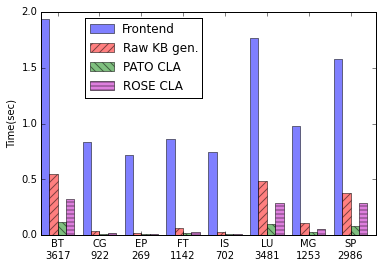
\includegraphics[width=.6\columnwidth]{graph/npb-cl.png}
	\caption{Time comparison of the canonical loop analysis. The
          X-axis shows the benchmark names and their numbers of
          source-code lines.}
	\label{fig:npb-cl}
\end{figure}


%Another advantage of the declarative approach is that the analysis rules can be added incrementally. To handle different cases for the same definition, we just need to add more rules without changing the existing ones. 
%It is seen that writing rules for program analysis is very productive in adding language feature support. 
%To cover more cases, we just need to add more rules in a very modular way. 
\noindent{\em Extensibility.} An appealing property of using ontology
is the good extensibility. The previous discussion only covers
canonical loops in C programs using primitive loop variable types,
such as pointer and integer types.  OpenMP allows C++ canonical loops
using complex iterator types for loop variables.
%For example, in the canonical loop specification, the \textsf{var} can be a variable of type random access iterator for C++. 
The iterator type must support random access---that is, allowing
element accesses using an arbitrary offset position relative to the
element they point to (offering a functionality similar to pointers).
%The random access iterator is an iterator that supports the access to elements in any order. 
%It provides 
%operations of ordinary C pointer arithmetic. 
Examples of random access iterators include \textsf{std::vector<T>::iterator} and \textsf{std::deque<T>::iterator}. % and ordinary pointers. 
Also, programmers often define their own random access iterators. 
%To support the CLA for C++, the analysis tools need to be able to recognize random access iterators. 
A conventional solution to extend an imperative CLA implementation is to store the known random access iterators, including the custom-defined ones, into a container for the compiler implementation to look-up. 
The solution is ad-hoc and it is not easy to exchange this knowledge with other tools or developers.

Ontology-based program analysis allows easy extensibility. 
In PATO, we can easily add the concept \textsf{RandomAccessIterator} in the language ontology and describe it logically as $\mathsf{is-a(Iterator)}\wedge\mathsf{has(RandomAcess)}$. 
The knowledge of \textsf{is-a(Iterator)} property can be gained by the knowledge builder while the knowledge \textsf{has(RandomAcess)} can be inserted into the knowledge base using the standard OWL API, either automatically by tools or manually by developers. 
The analysis rules can reason about the random access iterator logically. 
All the resulting ontology can be then shared and reused by different analyses.

\subsection{Control Flow Graph Construction}

The second program analyses we have developed on PATO is control flow
graph (CFG) construction. Different from the canonical loop analysis,
it requires the examination of control flows of the whole program.  On
PATO, it can be easily done through the set of simple rules.  by
following the algorithm of inductive graph
constructions~\cite{fischer_crafting_2009}.  The construction is
intuitive. For example, the rule to construct the CFG of a
\textsf{while}-statement is shown in Listing~\ref{code:cfg-prolog}.
\begin{lstlisting}[xleftmargin=.1\columnwidth,
xrightmargin=.1\columnwidth, escapechar=@, 
caption= Rule to construct CFG for a While statement, label=code:cfg-prolog]
cfg(@\emph{Stmt}@, @\emph{Entry}@, @\emph{Exit}@) :-
 isWhileStatement(@\emph{Stmt}@), !,
 hasCondition(@\emph{Stmt}@, @\emph{ConditionStmt}@),
 hasBody(@\emph{Stmt}@, @\emph{BodyStmt}@),
 @\emph{Entry}@ = @\emph{ConditionStmt}@,
 @\emph{Exit}@ = exit(@\emph{Stmt}@),
 cfg(@\emph{BodyStmt}@, @\emph{BodyEntry}@, @\emph{BodyExit}@),
 makeTrueEdge(@\emph{ConditionStmt}@, @\emph{BodyEntry}@),
 makeFalseEdge(@\emph{ConditionStmt}@, @\emph{Exit}@),
 makeEdge(@\emph{BodyExit}@, @\emph{ConditionStmt}@).
\end{lstlisting}

%This construction rule constructs CFG on per-statement level. 
The first clause in the body matches this rule with only the \textsf{while}-statement. 
The rest clauses find different components of the \textsf{while}-statement and construct the CFG nodes and edges. 
%according to Figure~\ref{fig:cfg}. 
%It is seen the process is very intuitive. 
A blank node (\textsf{exit(Stmt)}) is created to represent the exit node for the \textsf{while}-statement. 
The inductive construction for nested body statements are implemented by the recursive CFG rule \textsf{cfg(BodyStmt, ...)}.
%The per-statement CFG can be converted to basic block based CFG and the temporary blank nodes are removed. 
%\TODO{How to convert to basic block? Show the rules please.}
%Rules for different kind of statements are implemented separately and match the correct statements automatically.
The resulting CFG graph can be explicitly stored in ontology. 
We define relations like \textsf{hasNextEdge} to represent the directed edge in the CFG.
Nodes of CFG are just existing language construct entities in the program ontology.

\vspace*{.1in}\noindent {\bf Experimental Results} 
%\TODO{\sout{report comparison (lines of source code, analysis time, etc.)}}
For CFG analysis, we reuse the same initial knowledge base (originally generated to support the canonical loop analysis). 
%This shows the advantage of ontology-based program analysis -- the knowledge is easily shared and reused. Thus the overhead of building the knowledge is amortized over different analysis.
We compare our PATO implementation with the implementations of ROSE and Clang~\cite{lattner2008llvm}. 
%Both ROSE and Clang provide source level CFG analysis in their code base. 
%\TODO{what CFG construction algorithms are used in two compilers? Are the comparable to PATO's algorithm?}
Both ROSE and Clang implementations use the similar inductive construction algorithm but the details are different, especially the internal data structures. 
%Besides, ROSE and Clang support C++ while PATO doesn't support for now.
%Due to the difference of compiler implementation, it is difficult to do a strict comparison of code length. 

For productivity, we only measure the core code of the CFG analysis itself. % not including any dependency calls. 
Our goal is to find that if a specific analysis was not provided by the compiler, how many lines of codes are needed to implement it based on the existing APIs of the compiler. 
Source code comments and CFG printing statements are also excluded as much as possible to make the comparison fair.  
%The approximate line numbers are shown in Row 2 of Table~\ref{tbl:loc}. 
It turns out that the declarative approach uses only 400 lines of code, which is up to 8.75X more efficient than the traditional compiler implementations (1200 and 3500 lines for ROSE and Clang respectively).

The performance comparison is shown in Figure~\ref{fig:npb-cfg}.  The
time for PATO analysis doesn't include the knowledge building time.
Similarly, the time for ROSE and Clang analysis doesn't include their
frontend time.  The speed of the PATO analysis is as competitive as
imperative approaches due to the efficient storage and query of our
knowledge base.
%\TODO{Why ROSE's CFG is slowest? Please comment}
\begin{figure}[h]
	\centering
	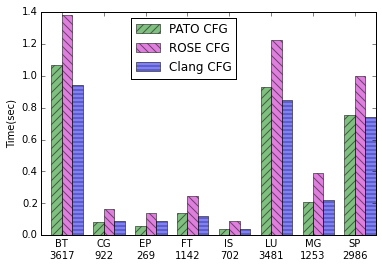
\includegraphics[width=.6\columnwidth]{graph/npb-cfg.png}
	\caption{Comparison of the analysis time taken by the three
          implementations for CFG construction.}
	\label{fig:npb-cfg}
\end{figure}

%%%%%%%%%%%%%%%%%%%%%%%%%%%%%%%%%%%%%%%%%%%%%%%%%%%%%%%%%%%%%%%%%%%%%%%%%%%%%%%
\subsection{Data Access Pattern Analysis}

%\TODO{One or two paragraphs to briefly explain what the analysis is and how it is implemented.}
The third analysis we have developed on PATO is data access pattern
analysis. Analyzing data access patterns is critical to many memory
optimizations (e.g., improving CPU cache
locality~\cite{kandemir1999improving}, enhancing GPU data
placement~\cite{Chen2014, Jang2011}.)  In our experiment, we
demonstrate how to use PATO to easily extract out data access patterns
from a CUDA (a GPU programming model from NVIDIA)~\cite{nvidia2011nvidia}
program.  Listing~\ref{code:dap-eg} shows an example
CUDA kernel executing a two level loop, where \textsf{f(tid,i,j)} is
an affine function about the thread index (\textsf{tid}) and loop
index. % (\textsf{i, j}).
\begin{lstlisting}[xleftmargin=.1\columnwidth,
xrightmargin=.1\columnwidth,
caption=An example CUDA kernel loop, label=code:dap-eg]
for(i=0;i<N;i++) {
 for(j=0;j<M;j++) {
  A[f(tid, i, j)]=B[...]+C[...]
 }
}
\end{lstlisting}

In this experiment, we define a data access pattern of an array as the
access expression (or called subscript expression) of that array in
each access, the lower and upper bounds of the loops surrounding the
accesses to that array, the number of reads and the number of writes
to that array, and the ranges of elements of the array being
accessed. Choosing such a definition is because a previous
work~\cite{Chen2014} has already implemented a C/C++ code in a
source-to-source compiler to extract the same set of
information. Using the same definition allows us to make a
head-to-head comparison.

Our experiment shows that with PATO, each of the types of
information can be easily extracted from the kernel code through just
a few lines of Prolog statements. For example, to obtain the index
range of arrays in a double nested loop as the arrays \textsf{A, B, C}
in Listing~\ref{code:dap-eg}, our query in Prolog is as follows:

\begin{lstlisting}[xleftmargin=.1\columnwidth,
xrightmargin=.1\columnwidth,escapechar=@, 
caption=An example query for finding data access patterns, label=code:dap]
accessPattern(@\emph{Array}@) :-
 arrayRef(@\emph{Array}@),
 inNestedLoops(@\emph{Array}@, @\emph{LoopList}@),
 getLoopTripCount(@\emph{LoopList}@, @\emph{LTCs}@),
 getIndex(@\emph{Array}@, @\emph{ArrayIndex}@),
 eval(@\emph{ArrayIndex}@, @\emph{LTCs}@).
\end{lstlisting}

The clauses in the query are high-level APIs provided by the PATO
framework. The first clause on the right hand side asks the reasoner
to find all instances in the ontology that belong to the class
\textsf{ArrayRef} (which is a defined concept in the ontology to
represent array references). The second clause checks each of those
instances to see whether it is in a nested loop. If so, it recursively
finds the enclosing loops from inner to outer and returns the loop
statements in the variable {\em LoopList}. The third clause stores the
loop trip counts (LTC) of those loops into {\em LTCs}---which can be
symbols or constants of the lower and upper bounds of the loop
indices. The fourth clause gets the array access expression, and the
final clause evaluates the expression with the loop trip counts info.
The support of symbolic manipulation in Prolog turns out to be handy
for this analysis. In rule~\ref{code:dap}, the LTC of a loop can be
evaluated using the symbolic expression feature of Prolog.  Assuming
the affine function in Listing~\ref{code:dap-eg} is $f(tid, i, j) = 64
* tid + 8 * i + j$.  If the thread number \textsf{nthreads},
\textsf{M} and \textsf{N} can be inferred, then the range of the
access is evaluated to concrete value.  Otherwise, the symbolic
expression ($64 * nthreads + 8 * M + N$) is captured for later use.
The knowledge of different access patterns are stored as normal
ontology triples like \textsf{(A hasAccessRange "(0,
  64*nthreads+8*M+N)")}.
%or \textsf{(A
%  hasAccess "written")}. 
%  \footnote{In practice, A is referred to by
%  IRI.}, which can be later easily queried.

%\TODO{How do you extract info. about read/write,  linear/stride/random using Prolog ?} 
%\vspace*{.1in}\noindent {\bf Experimental Results} 
%\TODO{report comparison (lines of source code, analysis time, etc.)}

%\subparagraph{Time performance comparison}
%\TODO{Time performance comparison is missing?} 

%\subparagraph{Productivity Comparison}
The previous imperative data access pattern
analysis~\cite{Chen2014} has more than 2000 lines of source code.
PATO, on the other hand, only needs 180 declarative rules to implement
the same analysis. We test both implementations on a set of GPU kernel code from the CUDA SDK (mentioned later) and
%(?? cite benchmark paper or URL ?? ). 
they get the same extraction results and take similar length of
analysis time. 
%The PATO version takes (??  more or less??) time than the imperative version does. 

%%%%%%%%%%%%%%%%%%%%%%%%%%%%%%%%%%%%%%%%%%%%%%%%%%%%%%%%%%%%%%%%%%%%%%%%%%%%%%%
\subsection{Data Placement Guidance}
%\TODO{Explain what the optimization is and how it is implemented in
%  this work in the rule-based and PORPLE approach; describe the
%  comparison with the previous PORPLE in terms of productivity and
%  extensibility when adding the support of a new type of memory; the
%  description can be based on the old 4.2; be more clear and concise.}
%se data placement optimization as an example to demonstrate the use of ontology-based analysis.
The fourth analysis also help test the promise of ontology-based
analysis for guiding program optimizations. The particular
optimization is called data placement optimization. It is to find the
suitable kinds of memory to place the data in a program. It is
important for devices with multiple types of memory having different
performance characteristics. An example is NVIDIA Graphic Processing
Units (GPU) as shown by previous studies~\cite{Chen2014, Jang2011}.
An important analysis to support the optimization is to find an
optimal placement strategy for a given program on a specific GPU.  We
define this analysis as {\em data placement guidance}.

This analysis needs not only the knowledge about the program (such as
data access pattern), but also hardware memory specifications in order
to make appropriate decisions.  In this study, we confirm that it is
natural to use ontology to express hardware knowledge as the knowledge
is just a set of attributes or relations of the different parts of the
device. Moreover, because both the program knowledge and the hardware
knowledge are represented in the standard three-tuple format, they can
be automatically linked into one single ontology to support auto
reasoning about data placement.

Previous work uses customized memory specifications.  For example, the
PORPLE framework \cite{Chen2014} features the memory specification
language (MSL) to communicate a memory system to compilers.
%The syntax of MSL for memory specification is shown in Listing~\ref{code:msl}.
%\begin{lstlisting}[caption=PORPLE MSL syntax, label=code:msl]
%memSpec ::= name id swmng rw dim size blockSize banks 
%latency upperLevels lowerLevels shareScope 
%concurrencyFactor serialCondition ; end-of-line
%\end{lstlisting}
Listing~\ref{code:msl} shows the syntax of MSL and an example
specification for the constant memory of Tesla M2075.

\begin{lstlisting}[basicstyle=\ttfamily\footnotesize, caption={PORPLE
      Memory Specification Language (? represents unknown attributes).}, label=code:msl]
% syntax 
memSpec ::= name id swmng rw dim size blockSize banks 
latency upperLevels lowerLevels shareScope 
concurrencyFactor serialCondition ; end-of-line
% an example 
constantMem 1 Y r na 64K  ? ? 360clk <cL2 cL1> <> die ? ... 
\end{lstlisting}
%which conforms to the syntax in Listing~\ref{code:msl} and interprets correspondingly.
%This specification provides the information about the device. 
The example specification represents the type of memory (constMem), a unique ID (in numbers),  whether the memory is software manageable (Y or N) and whether a GPU kernel can read or write the memory ("rw" filed). 
%The field “dim”, if not “?”, indicates that the spec entry is applicable only when the array dimensionality equals to the value of “dim”. 
The other fields indicate dimensionality, memory size, number of
banks, memory latency, and so on.  The disadvantage of MSL is that it is
only extensible for a new GPU with a similar architecture.  But for
new hardwares with new attributes not present in the MSL syntax, the
MSL syntax, as well as the ad-hoc parser requires significant
modification.

In the PATO system, the ontology representation is more generic and
extensible.  We don't need to design any specific syntax for hardware
knowledge.  Only new concepts and relations (or properties) in the
hardware domain need to be added. Figure~\ref{fig:gpu_onto}
illustrates part of the GPU ontology.
\begin{figure}[t]
	\centering
	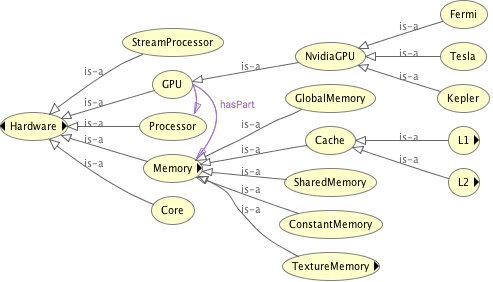
\includegraphics[width=.6\columnwidth]{graph/gpu_onto.jpg}
	\caption{Part of the GPU hardware ontology.}
	\label{fig:gpu_onto}
\end{figure}

Listing~\ref{ont:global_mem} shows the description of the
\textsf{Global Memory} on the Nvidia K20c GPU card.  The ontology
captures relations between the global memory and other components of
the GPU and also attributes of the memory.  It is expressive and easy
to extend. 
%In contrast, in PATO ontology representation, we just need to create new concepts for these new hardwares, new attributes and capture their relation with logic description.  
\begin{lstlisting}[xleftmargin=.05\columnwidth, 
xrightmargin=.05\columnwidth, float=h,
caption=Ontology of Tesla K20c global memory,label=ont:global_mem]
globalMem_k20c type GlobalMemory;
globalMem_k20c hasUpperLevel L2;
globalMem_k20c shareScope die;
globalMem_k20c pieces 1;
globalMem_k20c software_manageable true;
globalMem_k20c accessible "rw";
globalMem_k20c has_size 5032706048;
... % omitted
\end{lstlisting}

\vspace*{.1in}\noindent {\bf Guiding Data Placement}
Our experiment shows that with the ontology-based representation of
both program and hardware knowledge, it is easy to develop analysis to
guide the data placement optimization on GPU. 

Data placement guidance can rely on heuristic rules, mathematical
modeling, or their combinations.  For instance, a previous GPU
study~\cite{Jang2011} places data on GPU memory based on some
algorithms upon some empirical rules related with data access patterns
of arrays and the characteristics of different types of memory.  An
example rule is that constant memory is suitable for read-only data
which is small enough and satisfies the \emph{same address read}
condition (i.e., memory accesses to the array are the same across all
threads).  In another study named PORPLE~\cite{Chen2014}, analytical
cost models are used for finding good placements of data.  It
enumerates possible placement plans and estimates the cost of each
plan in terms of memory latency.  For each placement plan, it
coordinates all arrays together instead of placing them separately as
in the rule-based algorithm.
%PORPLE doesn't individually search for best memory for each array, but it considers all arrays and memories globally. 
%\TODO{wHAT does this mean? A single placement plan for all arrays?}

\begin{comment} % this looks too trivial to show in the paper
\begin{lstlisting}[caption=Top level rule for rule-based data placement, label=code:dp_rule]
suitablePlace(Array, Mem) :- 
 accessPattern(Array),
 suitableMem(Array, Mem). 
\end{lstlisting}
where the \textsf{getAccessPattern} is the rule of Listing~\ref{code:dap}. The \textsf{suitableMem} rule defines which memories are suitable for this array. 
\end{comment}

With PATO, it is easy to incorporate both the heuristic rules
and analytical models into an analysis for guiding data placement.
%This rule-based algorithm is straightforward to be implemented in PATO. 
For example, the logic rule to find suitable arrays for constant
memory can be expressed using Listing~\ref{code:dp_const}.
\begin{lstlisting}[xleftmargin=.05\columnwidth,
xrightmargin=.05\columnwidth,escapechar=@, 
caption=Rule for using constant memory, label=code:dp_const]
suitableMem(@\emph{Array}@, constantMem) :-
 readonly(@\emph{Array}@), 
 sizeFit(@\emph{Array}@, constantMem),
 sameAddressAccessWithinWarp(@\emph{Array}@).
\end{lstlisting}

Similarly, the algorithm used by PORPLE can be written as in
Listing~\ref{code:dp_model}.  The top-level rule \textsf{optimalPlace}
finds all the possible placement plans and estimates the cost of each
plan.  The \textsf{possiblePlacement} enumerates all possible plans.
(The rule-base placement algorithm (\textsf{suitableMem}) could be
plugged here to narrow down the search space.)  The estimation of the
cost of each placement is based on cache behaviors and is computing
intensive.  It is implemented as a {\em computable} (an external
procedure) and is hooked with the Prolog program through a special
clause (\textsf{call}).
%In line 17 of Listing~\ref{code:dp_model}, the \textsf{call} invokes the associated procedure for a query clause (\textsf{hasCost}).

\begin{lstlisting}[xleftmargin=.05\columnwidth,
xrightmargin=.05\columnwidth,escapechar=@, 
float=h, caption=Rules for PORPLE algorithm, label=code:dp_model]
optimalPlace(@\emph{BestPlacement}@) :-
 findall(@\emph{Placement}@, 
 (possiblePlacement(@\emph{Placement}@),
 hasCost(@\emph{Placement}@, @\emph{Cost}@)),
 Placements),
 minimalCost(@\emph{Placements}@, @\emph{BestPlacement}@).
 
possiblePlacement(@\emph{Placement}@) :-
 findall(Place,
 (isArray(@\emph{Array}@),
 suitableMem(@\emph{Array}@, @\emph{Mem}@),
 Place = place(@\emph{Array}@, @\emph{Mem}@)),
 Placement).
 
hasCost(@\emph{Placement}@, @\emph{Cost}@) :-
 hasCommand(hasCost, @\emph{Cmd}@),
 call(@\emph{Cmd}@, @\emph{Placement}@, @\emph{Cost}@).
\end{lstlisting}

\vspace*{.1in}\noindent {\bf Experimental Results} 
%\TODO{report the productivity and performance results}
We evaluate the PATO-based data placement guidance on a set of benchmarks. The \emph{mm, trans} kernels are from CUDA SDK and the \emph{particlefilter, spmv, cfd, mod} are from the RODINIA benchmark suite \cite{Che2009}.
We also choose two kernels \emph{glassForce, glassControl} from the DOE application LULESH (Cuda\_Fermi 1.0 version) \cite{LULESH1.0} to show the scalability of the data placer on large applications.
The machine used in the experiment is a desktop with Nvidia K20c GPU card and Intel Xeon E5-1607v2, host operating system is Linux-3.13 and the CUDA version is 6.5.

We use the rule-based and model-based data placement guidance to find
optimal data placement policies for the input tested kernels.  The
kernels using the new data placements are then measured for
performance.  The speedups over the original benchmarks are shown in
Figure~\ref{fig:dp_speedup}, agreeing with the speedups achieved
using the previous imperative implementation of the placement
analysis. The analysis time taken by PATO is on average 5\% longer
than the imperative implementations do.
%The PATO placer is based on PORPLE, we have manually verified the placement decision with PATO is the same with PORPLE.

\begin{figure}[ht]
	\centering
	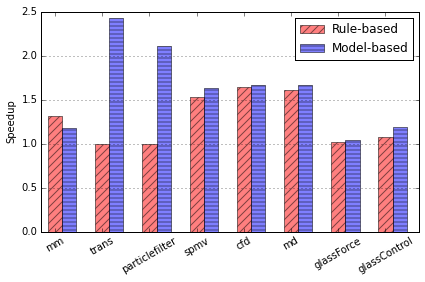
\includegraphics[width=0.6\columnwidth]{graph/dp_speedup}
	\caption{Speedup of benchmarks on Tesla K20c.}
	\label{fig:dp_speedup}
\end{figure}
%\TODO{replace PORPLE-based with model-based to contrast rule-based in the figure?}

% productivity
For productivity, PORPLE's parser for the custom MSL format written in
Python has approximately 270 lines while the ontology format can be
processed with standard libraries. The PORPLE framework is written in
an already compact scripting language, Python.  It still has about 950
lines code while the PATO implementation has about 380 lines.

% Extensibility
Compared to the alternatives, the PATO-based analyses are more
extensible and sharable due to their ontology representations and
declarative algorithms.  For example, in the previous approach used in
PORPLE, if knowledge about GPUs with new features is to be added, the
MSL format must be modified to add the corresponding fields; the code
for parsing MSL and querying the placement engine should be modified
as well.  In PATO, the changes are much easy to do. Through the Prolog
GUI, users can easily add or remove a concept. Analysis rules only
need to add queries for the features if needed.
%Besides, the PATO is more extensible in terms of productivity. For example, if a new kind of memory is added into the system, in the PORPLE, the \TODO{to be done}

%% % Overhead
%% Finally, we compare the analysis overhead of the PORPLE and PATO implementation in Figure~\ref{fig:dp_time_cmp}. 
%% The overhead is the time to run the data placement guidance algorithms, not the tested kernels. 
%% The result of \emph{glassForce} is not shown since its time is very large compared to others. 
%% The results show that the PATO's declarative implementation is comparable to the traditional imperative implementation in terms of time efficiency. 
%% The slowness is due to the overhead in PATO when the main Prolog programs call the external Python scripts calculating the cost of placement plans to answer the query \textsf{hasCost} in Listing~\ref{code:dp_model}.
%% %This overhead can be eliminated if we unify the program with one language.
%% \begin{figure}[ht]
%% 	\centering
%% 	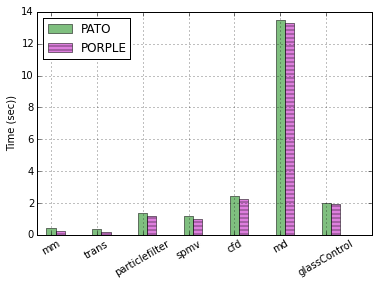
\includegraphics[width=0.7\columnwidth]{graph/dp_time_cmp}
%% 	\caption{Analysis overhead comparison}
%% 	\label{fig:dp_time_cmp}
%% \end{figure}
%% %\TODO{what is the agenda of this figure, which color is for which implementation?}

\subsection{Facilitating Cooperations}

\begin{figure}
	\centering 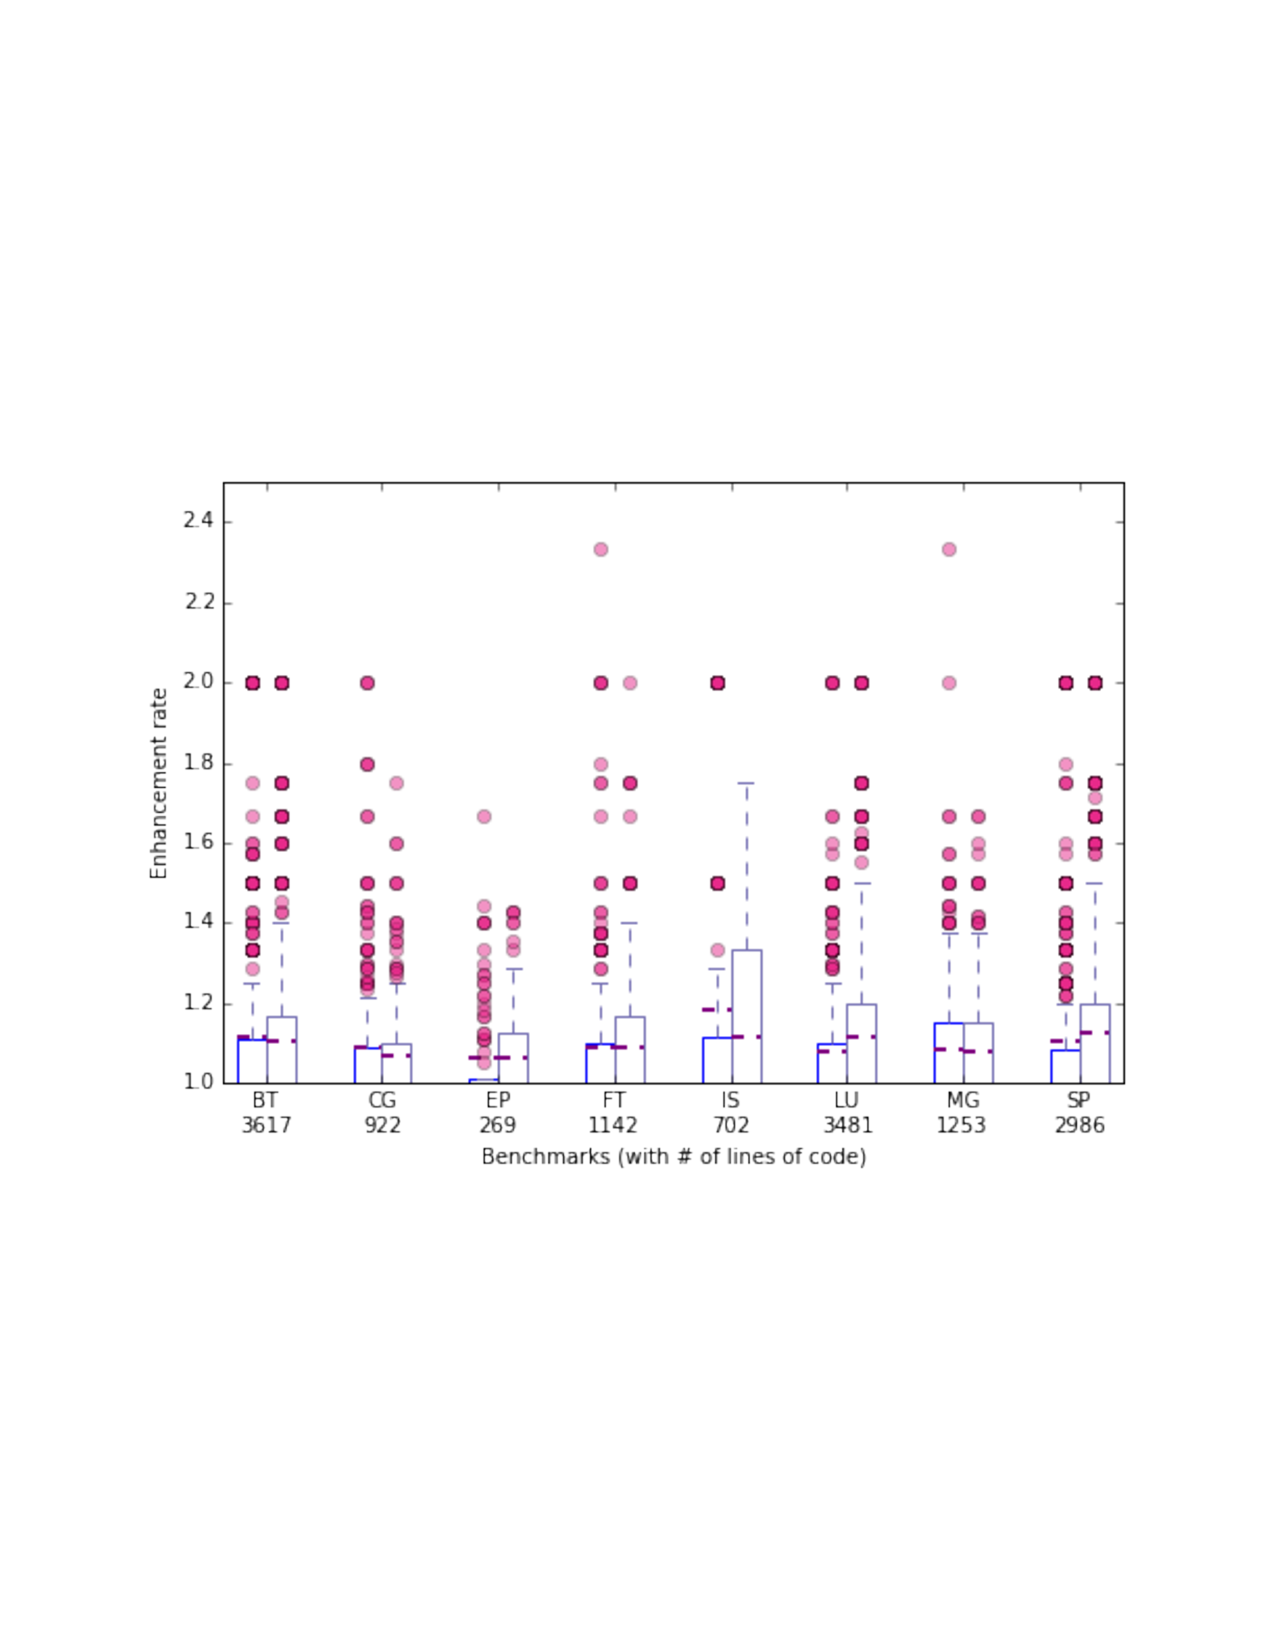
\includegraphics[width=0.6\columnwidth]{graph/lv_boxplot} \caption{Enhancement
	of Liveness analysis by leveraging ontology to combine the
	results from the Liveness analysis in LLVM Clang and
	ROSE. (Dots show outliers). Left bars: the enhancement over
	LLVM Clang results; right bars: the enhancement over ROSE
	results.}  \label{fig:coop}
\end{figure}

In the final experiment, we try to examine the potential benefits of
leveraging the standard representation of ontology to promote synergy
between different compilers. Particularly, we use Liveness analysis as
an example. 

As a {\em may-type} data flow analysis, Liveness analysis is
conservative---that is, if a variable belongs to the Liveout set of a
basic block, it means that the compiler cannot definitely tell that
the variable is dead at the end of the basic block. So, for two
different Liveness analyses (both are sound and conservative), if a
variable belongs to the result from one analysis but not that from the
other, we can conclude that that variable is not Live at the end of
the said basic block. In another word, the intersection of the results
of the two Liveness analyses gives a more precise result than either
of the two analyses. 

Both LLVM Clang and ROSE have their own Liveness analysis developed
before. By using the ontology converters we have developed for the two
compilers, we convert the Liveness analysis results from them into our
ontology. By writing several lines of Prolog code, the Prolog engine
immediately extracts out the intersection of the sets of Live
variables reported by the two compilers for each basic block of a
given program.

We define a metric called {\em enhancement rate} to characterize the
benefits of such a combination. Let A and B stand for two Liveness
analyses and $R_A$ and $R_B$ be their Liveout set for a given basic
block. The enhancement rate over $A$ is defined as

$enhancementRate(A) = \frac{|R_A|}{|R_A \cap R_B|}$

The enhancement rate over $B$ is defined similarly (with $A$ replaced with
$B$).

The results are shown in Figure~\ref{fig:coop}. Box plots are used to
show the distribution of the enhancement rates over all the basic
blocks in the program. The graph considers only the basic blocks whose
Liveout sets are not empty in the result from at least one of the two
compilers.  The results indicate that the synergy improves the average
precision of Liveness analysis by over 10\% and 20\% for LLVM Clang and ROSE
respectively.

It is worth noting that the two compilers use different internal
representations for programs and the Liveness analysis results. It is
possible to write some special code to map their results to enable
such a combination without using Ontology. However, using the ontology
designed in this work, the benefits come as simple side products of
the ontology-based program analysis (by leveraging the converters and
the standardized representation developed for many other program
analyses). The productivity benefits would become even more prominent
when many types of analyses cooperate across compilers.


\section{Related Work}
\label{sec:rel}
Ontology has been used to build various knowledge bases in
different domains, including biology~\cite{ashburner2000gene},
ambient
intelligence~\cite{ducatel2001scenarios,preuveneers2004towards,rodriguez2014survey},
robotics~\cite{tenorth2009knowrob}, and
others~\cite{matuszek2006introduction,niles2001towards,pease2002suggested}.
This work was enlightened by these studies, but concentrates on the
special challenges facing program analysis.

In the software domain, ontology has been introduced, but mainly for
software management and teaching of programming concepts, rather than
program analysis. Specifically, Software Ontology
(SWO)~\cite{malone2014software} in the domain of software engineering
focuses on the meta information of software (e.g., licenses,
publishing processes, data formats). COPS~\cite{lando2007towards}
offers a sub-ontology for managing the knowledge related with image
processing. Eden and others~\cite{eden2007problems} have provide some
theoretical discussions on the unique aspects in designing an ontology
for programs, but without exploring the use of ontology for program
analysis. There are several ontology designs for teaching some
programming
languages~\cite{sosnovsky2006development,ganapathi2011towards}.  This
current work, to our best knowledge, is the first proposal on a
systematic integration of ontology into program analysis, and PATO
is the first complete framework to do so.

There is some prior work trying to ease the difficulties in the
development of program analysis. OpenAnalysis~\cite{OpenAnalysis}
advocates the separation of analysis from the IR of a program to allow
the orthogonal development of compiler infrastructures and program
analysis. Several other studies have tried to store some program
components and relations in relational databases and they use logic
programming to do program
analysis~\cite{hajiyev2006codequest,bravenboer2009strictly,whaley2005using}.
These work demonstrates some promising results on some specific tasks
(e.g., points-to analysis). 

The representations used in those work are in some customized format
tied closely to some low-level form of the program (e.g., Java byte
code~\cite{benton2007interactive}). Compared to ontology---a generic
way for knowledge representation, they are subject to some principled
limitations as the three limitations mentioned in the introduction
section. For instance, they cannot be used to represent other types of
knowledge that could be relevant to program analysis. An example is
the GPU memory properties Section~\ref{sec:exp} describes for guiding
data placement on the GPU. To apply the previous methods to that task,
one has to design some additional ways to represent such hardware
knowledge and develop much additional code to manipulate it and
integrate it into the program analysis framework. These extra work
largely throttles the productivity benefits of those methods. In
comparison, ontology-based analysis allows a seamless integration of
the hardware knowledge in the knowledge base, making it possible for
the existing reasoning engine to automatically reason about data
placements. It further eases the support of cooperations between different
compilers and analysis tools, and avoids the many efforts in
developing a preprocessing for each program analysis. 

% intuitive
% generic
% auto inference
% ecosystem


\section{Conclusion}
\label{sec:conc}
This work demonstrates the promise of ontology for overcoming the
three major limitations of today's declarative program analysis. The
four types of data analyses on PATO show that the single ontology is
able to support multiple different program analyses efficiently. The
GPU data placement experiments indicate the promise of ontology for
seamlessly linking knowledge from different sources, extending
declarative program analysis with the capability to effectively guide
program optimizations. The cooperative Liveness analysis demonstrates
that with ontology-based program analysis, cooperations among
different compilers or other program analysis tools become simple, and
the synergy turns out to be quite beneficial. Overall, the study shows
some good promise of the integration of Ontology into program
analysis. We hope that this work will prompt further investigations by
the community into this promising direction, and stimulate some
discussions in this new paradigm of program analysis.


%\nocite{Simpson}
\bibliographystyle{plain}% the recommended bibstyle
\bibliography{references,semantics,rose,knowledge}
	
	
\end{document}

